\documentclass[11pt]{article}
\input{glyphtounicode}
\input{glyphtounicode-cmex}
\pdfgentounicode=1
\pdfglyphtounicode{negationslash}{0338}
\usepackage[T1]{fontenc}
\usepackage{lmodern}
\usepackage[a4paper,margin=30mm]{geometry}
\usepackage{amsmath,amssymb,amsthm,mathtools}
\usepackage{microtype}
\usepackage{needspace}
\usepackage{tikz}
\usetikzlibrary{arrows.meta,calc,positioning}
\usepackage{float}
\usepackage[hyphens]{url}
\usepackage[colorlinks=true,linkcolor=blue!45!black,citecolor=blue!45!black,urlcolor=blue!45!black]{hyperref}
\hypersetup{pdftitle={Brennan's conjecture and sharp inverse-square integral means},pdfauthor={OpenAI}}
\pdfinfoomitdate=1
\pdftrailerid{}
\pdfsuppressptexinfo=15
\newcommand{\HH}{\mathbb H}
\newcommand{\DD}{\mathbb D}
\newcommand{\CC}{\mathbb C}
\newcommand{\KK}{\mathcal K}
\newcommand{\SSS}{\mathcal S}
\newcommand{\EE}{\mathbb E}
\newcommand{\dd}{\,d}
\DeclareMathOperator{\supp}{supp}
\DeclareMathOperator{\Rea}{Re}
\DeclareMathOperator{\Ima}{Im}
\newtheorem{theorem}{Theorem}[section]
\newtheorem{proposition}[theorem]{Proposition}
\newtheorem{lemma}[theorem]{Lemma}
\newtheorem{corollary}[theorem]{Corollary}
\theoremstyle{definition}
\newtheorem{definition}[theorem]{Definition}
\theoremstyle{remark}
\newtheorem{remark}[theorem]{Remark}
\numberwithin{equation}{section}
\title{Brennan's conjecture and sharp inverse-square integral means}
\author{OpenAI}
\date{September 24, 2026}
\begin{document}
\maketitle
\begin{abstract}
We prove Brennan's conjecture: if a simply connected plane domain admits a
conformal bijection $\varphi$ onto the unit disk, then $|\varphi'|^s$ is
area-integrable for every $4/3<s<4$. We also prove the sharp inverse-square
integral-means exponent $B_{\SSS}(-2)=1$ for the normalized schlicht class
$\SSS$.
\end{abstract}
\tableofcontents
\section{Introduction}
\label{sec:introduction}

Let $\DD=\{z\in\CC:|z|<1\}$, and write $dA=dx\,dy$ for planar
Lebesgue measure. A domain is a connected open subset of $\CC$; a
univalent map is an injective holomorphic map. Brennan's conjecture asks
whether, for every conformal bijection $\varphi:W\to\DD$ from a simply
connected plane domain, the derivative satisfies
\[
 \int_W|\varphi'(z)|^s\dd A(z)<\infty
 \qquad\left(\frac43<s<4\right).
\]
There is no regularity assumption on the boundary and no boundedness
assumption on $W$. The problem measures how strongly a conformal map can
compress area near an arbitrary boundary. The conjecture dates to
Brennan's 1978 work \cite{Brennan1978}; the domain and integral-means
formulations are recorded in \cite[Chapter~3]{Bertilsson1999}.

The inverse map $f=\varphi^{-1}:\DD\to W$ puts all source domains on
the same footing. Conformal change of variables gives
\begin{equation}\label{eq:inverse-area}
 \int_W|\varphi'|^s\dd A
 =\int_{\DD}|f'|^{2-s}\dd A.
\end{equation}
Thus the conjectured interval becomes $-2<t<2/3$, with $t=2-s$.
Positive powers detect large derivatives, whereas the difficult negative
powers detect small derivatives. The inverse-square power $t=-2$ is
the limiting case relevant to the upper endpoint $s=4$.

To state its radial form, let
\[
 \SSS=\{f:\DD\to\CC\text{ univalent}:f(0)=0,\ f'(0)=1\}
\]
be the normalized schlicht class. For $f\in\SSS$, $t\in\mathbb R$,
and $0<r<1$, define
\[
 M_t[f'](r)=\frac1{2\pi}\int_{-\pi}^{\pi}
                  |f'(re^{i\theta})|^t\dd\theta,
\]
and put
\begin{align*}
 \beta_f(t)&=\limsup_{r\uparrow1}
       \frac{\log M_t[f'](r)}{\log(1/(1-r))},\\
 B_{\SSS}(t)&=\sup_{f\in\SSS}\beta_f(t).
\end{align*}
Equivalently, $\beta_f(t)$ is the infimum of the real $b$ for which
$M_t[f'](r)=O((1-r)^{-b})$ as $r\uparrow1$; the implicit constant may
depend on $f$. In particular, the supremum defining $B_{\SSS}$ is taken after forming
each map's limiting exponent. We prove the following uniform estimate
directly, and then derive the area assertion.

\begin{theorem}[Brennan's conjecture and inverse-square means]
\label{thm:main}
For every $\varepsilon>0$ there is $C_\varepsilon<\infty$ such that
\begin{equation}\label{eq:main-uniform}
 M_{-2}[f'](r)\le C_\varepsilon(1-r)^{-1-\varepsilon}
 \qquad\left(f\in\SSS,\ \frac12\le r<1\right).
\end{equation}
Moreover, $B_{\SSS}(-2)=1$.

Let $W\subset\CC$ be any simply connected domain whose boundary in
the Riemann sphere contains at least two points. Every conformal
bijection $\varphi:W\to\DD$ satisfies
\[
 \int_W|\varphi'(z)|^s\dd A(z)<\infty
 \qquad\left(\frac43<s<4\right).
\]
Equivalently, every univalent map $f:\DD\to\CC$ satisfies
\[
 \int_{\DD}|f'(w)|^t\dd A(w)<\infty
 \qquad\left(-2<t<\frac23\right).
\]
\end{theorem}

The domain correspondence, including the boundary condition, is
justified in Section~\ref{sec:integrability}. That section also derives
$B_{\SSS}(t)=|t|-1$ for every $t\le-2$; the corresponding uniform
radial bounds retain an arbitrary positive loss. The radial exponent $1$
is compatible with divergence of the area integral at $t=-2$.
The other area endpoint also fails for the same classical example.

\begin{corollary}[Sharpness of the open range]\label{cor:sharp-endpoints}
The Koebe function $f(z)=z/(1-z)^2$ belongs to $\SSS$ and satisfies
\[
 \int_{\DD}|f'|^{-2}\dd A=\infty,
 \qquad
 \int_{\DD}|f'|^{2/3}\dd A=\infty.
\]
Its inverse therefore fails area integrability at both $s=4$ and $s=4/3$.
\end{corollary}

\subsection{The problem and its development}

Brennan's 1978 work \cite{Brennan1978,Brennan1978LOMI} improved the
previously known upper range beyond $s=3$, as recorded in
Bertilsson's historical account \cite[Chapter~3, pp.~43--44]{Bertilsson1999}.
The standard formulation asks for the full interval $4/3<s<4$ on every
simply connected plane domain admitting a conformal bijection to the disk.
Neither boundedness nor boundary regularity is imposed. The classical
slit-plane obstructions at both endpoints are verified in
Section~\ref{sec:integrability}.

Subsequent progress connected the area question to finer estimates for
derivative integral means. Pommerenke developed this approach in
\cite{Pommerenke1985IntegralMeans,Pommerenke1985IntegralMeansII}.
Carleson and Makarov related negative integral means to the distribution
of large harmonic measure and proved the linear spectral tail
$B_{\SSS}(t)=|t|-1$ for all sufficiently negative $t$
\cite[\S1.4]{CarlesonMakarov1994}. The proposed threshold $t=-2$
is the one associated with Brennan's conjecture
\cite{HedenmalmShimorin2005}. The statement for sufficiently negative parameters alone
does not reach that endpoint.

Bertilsson studied coefficient estimates for negative powers of
derivatives of univalent functions \cite{Bertilsson1998}. His thesis
reports the area range $4/3<s<3.421$ \cite{Bertilsson1999} and
establishes equivalences between the spectral endpoint and
uniform integral-means formulations
\cite[Theorem~3.7, especially parts (a) and (f), pp.~44--45]{Bertilsson1999}.
Thus uniform estimates have an established place in the formulation of
Brennan's problem. In the present argument, the common constant in
\eqref{eq:main-uniform} arises directly from an operator on the entire
compact normalized class.

Hedenmalm and Shimorin combined area inequalities with weighted Bergman
space methods to improve general bounds for the integral-means spectrum.
Their published table gives $B_{\SSS}(-2)\le1.218$
\cite[Table~1, p.~385]{HedenmalmShimorin2005}.
Sola extended the Bergman-space computation
\cite{Sola2006}, reporting the improved estimate
$B_{\SSS}(-2)\le1.206$ in his thesis \cite[p.~6]{Sola2007Thesis}.
These estimates illustrate the remaining gap between general analytic
bounds and the conjectured exponent $1$.

Recent works treat the conjectured integrability range under additional
hypotheses. Aleman and Kouroupis prove it for members of continuous
semigroups of conformal disk self-maps and for Koenigs maps of nontrivial
such semigroups
\cite[Theorem~1.1 and Proposition~2.2]{AlemanKouroupis2025}.
Zheng treats simply connected polynomial basins at infinity for
$P(z)=z^m+a_0$, $m\ge3$, and for monic degree-$m$ polynomials whose
coefficients of $z,\ldots,z^{m-1}$ have modulus smaller than a
degree-dependent threshold; these basins
are considered in the sphere and contain infinity
\cite[Theorems~1.3--1.4]{Zheng2026Basins}.
Jin computes the real integral-means spectra of normalized rational
functions univalent in the disk,
with inverse-square supremum $1$ over that class
\cite[Theorem~6.20 and Corollaries~6.22--6.23]{Jin2025IntegralMeans}.
His work on Schwarzian multiplication operators recalls Shimorin's
sufficient multiplier-norm criterion for the inverse-square endpoint
of an individual normalized univalent function
\cite[Proposition~1.4(2)]{Jin2026Multipliers}.
Theorem~\ref{thm:main} concerns the full class of univalent disk maps.

\subsection{Analytic and geometric ingredients}

Normalized changes of base point, distortion estimates, and compactness
of the schlicht class are classical tools of geometric function theory
\cite[Chapters~1--2]{Duren1983}. A related probabilistic method for
exterior integral means appears in the conformal snowflakes of Beliaev
and Smirnov. Their positive integral operator gives lower bounds for an
averaged exponent defined from expected derivative integral means.
For each real $t$ and $\varepsilon>0$, they construct a random snowflake
whose averaged exponent exceeds $B(t)-\varepsilon$, where $B$ is their
universal spectrum defined using exterior Riemann maps
\cite[Lemma~3.4 and Theorem~4.1]{BeliaevSmirnov2010}.
Here the operator acts on all normalized half-plane maps, and
hypothetical excess growth produces a weighted affine law. The
operator is defined in Section~\ref{sec:preliminaries};
Section~\ref{sec:weighted-law} constructs its eigenmeasure and proves
the averaging identity.

The critical-point comparison is a planar index argument. Its
boundary calculation uses Hopf's secant proof of the tangent-turning
theorem \cite[\S2, pp.~53--55]{Hopf1935}, while the regular-target
step is an elementary plane case of Sard's theorem
\cite[Theorem~4.1]{Sard1942}.
We keep the index of a possible pole separate from those of the finite
critical points. The pairing is defined by ranks in ordered lists;
its measurability is proved through continuous local inverse branches,
and its equivariance follows from the ordering itself.

The subsequent area comparison is related in form to equivariant
mass transport, including the general framework for nonunimodular
group actions developed by Gentner and Last \cite{GentnerLast2011}.
We use a direct calculation with local changes of variables and
explicit expanding boxes. The affine covariance, exceptional-target
transfer, and boundary-cost estimates needed here are all proved
within the paper.

An independent companion applies a related affine-law and critical-point
comparison to prove a uniform inverse-first-power bound with exponent
strictly below $1/4$ for normalized univalent disk maps, disproving
Kraetzer's bounded-spectrum prediction at $p=-1$
\cite[Theorem~1.1]{OpenAIStrictInverseFirst2026}.
The proof here does not use that strict estimate; its H\"older
interpolation from \eqref{eq:main-uniform} gives exponent $1/2$ with
an arbitrary positive loss at $t=-1$.


\subsection{The obstacle and the proof strategy}

The classical distortion theorem bounds $|f'(z)|^{-1}$ by a constant
times $(1-|z|)^{-1}$ for $f\in\SSS$. Squaring this estimate gives
radial growth with exponent $2$, while the required exponent is $1$.
The missing information concerns how often very small derivatives can
occur around a circle. Our proof encodes hypothetical excess growth in
a probability law on conformal maps. That law imposes an algebraic sign
on an expected Jacobian; a geometric pairing of critical points imposes
the opposite sign.

We work on the upper half-plane $\HH=\{x+iy:y>0\}$ with the compact
class $\KK$ of univalent maps $F$ normalized by $F(i)=0$ and $F'(i)=1$.
Write $Q_F=1/F'$. Changing the base point to $z=x+iy$ gives
\[
 T_zF(w)=\frac{F(x+yw)-F(x+iy)}{yF'(x+iy)}.
\]
Each $T_zF$ again belongs to $\KK$. A positive operator averages the
two changes of base point $z=\pm1/2+i/2$, with weights $|Q_F(z)|^2$.
Its iterates sample equally spaced points above a fixed interval at
dyadic heights. If $\rho$ denotes the exponential growth rate of their
operator norms, Section~\ref{sec:preliminaries} shows that $\rho\le2$
implies the uniform disk estimate in Theorem~\ref{thm:main}.

Suppose instead that $\rho>2$, and put $\beta=\log_2\rho>1$.
Section~\ref{sec:weighted-law} constructs a Borel probability law $P$
on $\KK$ with the following property: for every $x+iy\in\HH$ and
every nonnegative Borel function $\Phi$ on $\KK$,
\[
 \mathbb E_P\bigl[|Q_F(x+iy)|^2\Phi(T_{x+iy}F)\bigr]
       =y^{-\beta}\mathbb E_P\Phi(F).
\]
We first construct a positive eigenmeasure, then average horizontal
translations and logarithmic scales. The resulting identity holds at
every affine change of base point. Differentiating the constant-test
identity determines the moments of the logarithmic derivative that
will control the Jacobian.

For $\xi\in\CC$, consider the target potential
\[
 V_\xi^F(x+iy)=\frac{y^k}{|F(x+iy)-\xi|},
 \qquad k=\frac{\beta+3}{4}>1.
\]
At the unique possible preimage of $\xi$ we give it value $+\infty$.
A critical-point count is useful only if points above a fixed positive
level cannot escape to the real axis or to infinity. Section~\ref{sec:escape}
proves precisely this compactness for almost every target and almost
every sampled map. The main boundary estimate controls the total length
of a horizontal line mapped into a compact target set.

The critical points of $V_\xi^F$ solve
\[
 G_F(z)=\xi,\qquad G_F(x+iy)=F(x+iy)-\frac{iy}{k}F'(x+iy).
\]
Section~\ref{sec:critical-pairing} shows that the sign of the normalized
real Jacobian of $G_F$ distinguishes saddles from maxima when $\xi$
is a regular value. For these targets, an index count on compact
superlevel boundaries gives at least as many maxima as saddles above
each positive level. Ordering the two lists by their values of $V_\xi^F$
therefore pairs each saddle with a distinct maximum of at least the
same value. We prove that this assignment is Borel and respects every
affine change of source coordinates. These properties are essential
when the pointwise pairing is integrated against $P$.

Section~\ref{sec:transport} performs that integration. Change of
variables through $G_F$ converts a weighted source area into the target
weight $(V_\xi^F/k)^4$. The pairing increases this weight. Affine
covariance then turns the expected source density into $dx\,dy/y$;
expanding boxes have asymptotically negligible boundary enlargement.
This proves that the expected normalized Jacobian is nonpositive,
contradicting its strictly positive value from the logarithmic-derivative
moments. A separate application of the same area formula handles the
exceptional targets at the distinguished point $i$, whose target
$G_F(i)=-i/k$ is fixed by normalization.

Finally, Section~\ref{sec:integrability} obtains the negative area
exponents $-2<t<0$ by H\"older's inequality and treats the positive exponents
with classical growth estimates and a weighted area argument. It
also proves the equivalence with the endpoint spectrum and the Koebe
sharpness assertions. Thus the analytic law, the compactness of
superlevels, and the measurable pairing each supply a distinct input
to the same weighted area contradiction.

\section{Univalent maps and a dyadic transfer operator}
\label{sec:preliminaries}

We first place normalized univalent maps of the upper half-plane in a
compact space.  Rescaling the source about a point then defines a positive
operator weighted by the inverse square of the derivative.  The main
conclusion of this section is a uniform comparison between powers of that
operator and disk integral means.  Later sections will bound the operator's
growth rate.

\subsection{Classical estimates and the normalized compact class}

We use the classical coefficient, distortion, growth, and quarter-disk
estimates in the following precise forms; see Duren
\cite[Chapter~2, especially \S2.3]{Duren1983}. No boundary regularity
or boundedness of the image is required.

\Needspace{12\baselineskip}
\begin{lemma}[Classical univalence estimates]
\label{lem:classical-univalence}
If $f(z)=z+a_2z^2+\cdots$ belongs to $\SSS$, then $|a_2|\le2$ and,
for $|z|=r<1$,
\begin{equation}
 \frac{1-r}{(1+r)^3}\le |f'(z)|\le\frac{1+r}{(1-r)^3},
 \qquad \frac r4\le |f(z)|\le\frac{r}{(1-r)^2}.
 \label{prelim:disk-bounds}
\end{equation}
Every univalent holomorphic map $g$ on an open disk $B(z_0,R)$ satisfies
\begin{equation}
 B\bigl(g(z_0),R|g'(z_0)|/4\bigr)\subset g(B(z_0,R)).
 \label{prelim:quarter}
\end{equation}
\end{lemma}

\begin{proof}
The coefficient and derivative bounds are the classical estimates just
cited. The classical lower growth bound $r/(1+r)^2$ implies the weaker
bound $r/4$ recorded here. A univalent holomorphic map has nonzero
derivative, so for the last assertion the map
\[
 \zeta\longmapsto
 \frac{g(z_0+R\zeta)-g(z_0)}{R g'(z_0)}
\]
belongs to $\SSS$. Applying the Koebe quarter theorem to this normalized
map gives \eqref{prelim:quarter}.
\end{proof}

Write
\[
 \HH=\{x+iy:x\in\mathbb R,\ y>0\},\qquad
 m(z)=\frac{z-i}{z+i},
\]
and let
\[
 \KK=\{F:\HH\to\CC\text{ univalent}:F(i)=0,\ F'(i)=1\}.
\]
We give $\KK$ the topology of locally uniform convergence.  Since
$m'(i)=1/(2i)$, its correspondence with the disk class is exactly
\begin{equation}
 F(z)=2i f(m(z)),\qquad
 f(\zeta)=\frac{F(m^{-1}(\zeta))}{2i}.
 \label{prelim:normalization}
\end{equation}
For $F\in\KK$, define the holomorphic function
\[
 Q_F(z)=\frac1{F'(z)}.
\]

\begin{lemma}[Compactness and uniform local bounds]
\label{lem:compact-class}
The space $\KK$ is compact and metrizable.  For every integer $j\ge0$,
the evaluations $(F,z)\mapsto F^{(j)}(z)$ and
$(F,z)\mapsto Q_F^{(j)}(z)$ are jointly continuous on $\KK\times\HH$
and bounded on $\KK\times E$ for every compact $E\subset\HH$.
For every $C_0\ge0$,
\begin{equation}
 |Q_F(x+iy)|\le\frac{(C_0^2+4)^2}{y}
 \quad\bigl(F\in\KK,\ |x|\le C_0,\ 0<y\le1\bigr).
 \label{prelim:strip-bound}
\end{equation}
In particular the bound is $64/y$ when $|x|\le2$.  Also,
\begin{equation}
 |F(z)|\ge\frac1{16}
 \quad\text{if }F\in\KK\text{ and }|m(z)|\ge\frac12.
 \label{prelim:zero-separation}
\end{equation}
\end{lemma}

\begin{proof}
The upper growth bound and \eqref{prelim:normalization} give local uniform
boundedness.  Montel's theorem therefore gives a locally uniformly
convergent subsequence from every sequence in $\KK$; see
\cite[Sections~1.1 and~1.3]{Duren1983} for this normal-family argument and
the univalent-limit form of Hurwitz's theorem.  Cauchy's formula preserves
the derivative normalization, so a limit $F$ has $F'(i)=1$ and is
nonconstant.  For any fixed $z_0\in\HH$, apply Hurwitz's theorem to
$F_n(z)-F_n(z_0)$ on the connected domain $\HH\setminus\{z_0\}$.
The limit is not identically zero and has no zero there.  Thus $F$ is
injective and belongs to $\KK$.  The compact-open topology is metrizable
using a countable compact exhaustion of $\HH$, so this sequential
compactness proves compactness.

Cauchy's formula gives locally uniform convergence of all derivatives.
The limiting derivative is nonzero, so reciprocals also converge locally
uniformly, as do their derivatives.  These observations give the asserted
joint continuity.  Compactness of $\KK\times E$ then gives the uniform
bounds.

For the explicit estimate, put $D=|x+i(y+1)|^2$ and $r=|m(x+iy)|$.
Then
\[
 1-r^2=\frac{4y}{D},\qquad
 |Q_F(x+iy)|=\frac{D}{4|f'(m(x+iy))|}.
\]
The lower derivative bound in \eqref{prelim:disk-bounds} gives
\[
 |Q_F(x+iy)|
 \le\frac{D(1+r)^3}{4(1-r)}
 =\frac{D^2(1+r)^4}{16y}
 \le\frac{D^2}{y}.
\]
When $|x|\le C_0$ and $y\le1$, this proves
\eqref{prelim:strip-bound}.

Finally $|m(z)|<1/7$ on $B(i,1/4)$, while
\eqref{prelim:quarter} gives
$B(0,1/16)\subset F(B(i,1/4))$.  Injectivity prevents any point outside
$B(i,1/4)$ from having an image of modulus less than $1/16$.  This proves
\eqref{prelim:zero-separation}.
\end{proof}

\subsection{Affine rescaling and dyadic growth}

Identify $z=x+iy\in\HH$ with the affine map $w\mapsto x+yw$.
Composition of these source maps is the product
\begin{equation}
 z\cdot w=x+yw,
 \qquad z^\#=\frac{-x+i}{y},
 \label{prelim:affine-product}
\end{equation}
with identity $i$ and inverse $z^\#$.  For $F\in\KK$ define
\begin{equation}
 T_zF(w)=\frac{F(z\cdot w)-F(z)}{yF'(z)}.
 \label{prelim:rerooting}
\end{equation}
It belongs to $\KK$.  On the space $C(\KK)$ of continuous
complex-valued functions, equipped with its supremum norm, define
\begin{equation}
 A_z\Phi(F)=|Q_F(z)|^2\Phi(T_zF),\qquad
 L=\frac12\bigl(A_{-1/2+i/2}+A_{1/2+i/2}\bigr).
 \label{prelim:operators}
\end{equation}
An operator is called positive here if it takes nonnegative real-valued
functions to nonnegative functions.  The operators in
\eqref{prelim:operators} are positive.  Their weights measure how the
inverse derivative changes when the source is rescaled.

\begin{lemma}[Affine identities and transfer growth]
\label{lem:transfer-growth}
For $z,w\in\HH$ and $F\in\KK$,
\begin{equation}
 Q_{T_zF}(w)=\frac{Q_F(z\cdot w)}{Q_F(z)},\qquad
 T_w(T_zF)=T_{z\cdot w}F,\qquad A_zA_w=A_{z\cdot w}.
 \label{prelim:composition}
\end{equation}
Each $A_z$ is bounded on $C(\KK)$, and for fixed $\Phi\in C(\KK)$
the map $z\mapsto A_z\Phi$ is continuous in the supremum norm.
For $n\ge0$, put $v_n=2^{-n}$ and
$u_{n,j}=-1+(2j+1)v_n$, $0\le j<2^n$.  Then
\begin{equation}
 L^n=v_n\sum_{j=0}^{2^n-1} A_{u_{n,j}+iv_n},\qquad
 \|L^n\|=\max_{F\in\KK}L^n\mathbf1(F).
 \label{prelim:dyadic-grid}
\end{equation}
The limit
\begin{equation}
 \rho=\lim_{n\to\infty}\|L^n\|^{1/n}
      =\inf_{n\ge1}\|L^n\|^{1/n}
 \label{prelim:rho}
\end{equation}
exists and satisfies $1\le\rho\le4$.  If $\lambda>\rho$, there is
$C_\lambda<\infty$ such that $\|L^n\|\le C_\lambda\lambda^n$ for
all $n\ge0$.
\end{lemma}

\begin{proof}
Differentiating \eqref{prelim:rerooting} proves the first identity in
\eqref{prelim:composition}.  Applying the normalization twice proves
the second.  In the operator product the weights telescope:
\[
 |Q_F(z)|^2|Q_{T_zF}(w)|^2=|Q_F(z\cdot w)|^2.
\]
This gives the third identity, with its displayed order of multiplication.
Joint continuity of $(z,F)\mapsto T_zF$ follows from locally uniform
convergence on affine images of compact source sets and the nonzero
normalizing denominator.  Together with Lemma~\ref{lem:compact-class},
this proves boundedness of $A_z$.  For fixed $\Phi$, joint continuity
on $\KK$ times a compact neighborhood of $z$ gives the asserted
supremum-norm continuity.

A word of length $n$ in the affine maps $-1/2+i/2$ and $1/2+i/2$
has height $2^{-n}$ and real part
$\sum_{l=1}^n\sigma_l2^{-l}$, where $\sigma_l\in\{-1,1\}$.
Writing $\sigma_l=2\epsilon_l-1$ and
$j=\sum_{l=1}^n\epsilon_l2^{n-l}$ gives real part
$-1+(2j+1)2^{-n}$.  Each $j$ occurs once and each word has coefficient
$2^{-n}$.  Expansion of $L^n$ proves the grid formula; at $n=0$ it
reduces to $A_i=I$.

For the positive sums defining $L^n$,
\[
 |L^n\Phi|\le L^n|\Phi|\le\|\Phi\|_\infty L^n\mathbf1.
\]
Testing with $\Phi=\mathbf1$ proves the norm identity.  At the map
$F(z)=z-i$ every summand in $L^n\mathbf1(F)$ equals one, so
$\|L^n\|\ge1$.  Since $|u_{n,j}|\le1$,
\eqref{prelim:strip-bound} gives
\[
 \|L^n\|\le625\,4^n.
\]
The logarithms of these positive norms are subadditive.  More explicitly,
for fixed $N\ge1$ write $n=qN+r$, $0\le r<N$, and use
$\|L^n\|\le\|L^N\|^q\|L^r\|$.  Taking the upper limit of the
$n$th roots and then the infimum over $N$ proves
\eqref{prelim:rho}; the displayed lower and upper bounds give
$1\le\rho\le4$.  If $\lambda>\rho$, the root limit bounds
$\|L^n\|$ by $\lambda^n$ for all sufficiently large $n$.  Increasing
a constant to cover the finitely many remaining $n$ proves the last claim.
\end{proof}

\subsection{From dyadic samples to disk integral means}

The next proposition explains why an upper bound on $\rho$ controls an
entire circle.  The comparison uses the same compact family in every
cell, so all its constants are independent of the chosen univalent map.

\begin{proposition}[Uniform disk comparison]
\label{prop:disk-transfer}
If $\rho\le2$, then for every $\varepsilon>0$ there is
$C_\varepsilon<\infty$ such that
\begin{equation}
 M_{-2}[f'](r)\le C_\varepsilon(1-r)^{-1-\varepsilon}
 \quad\bigl(f\in\SSS,\ 1/2\le r<1\bigr).
 \label{prelim:uniform-disk}
\end{equation}
The constant depends only on $\varepsilon$.
\end{proposition}

\begin{proof}
Fix $f\in\SSS$ and $1/2\le r<1$.  Put $\delta=1-r$ and choose
$n\ge1$ with $v=2^{-n}\le\delta<2v$.  On the fixed angular interval
$I=[3\pi/4,5\pi/4]$, write
\[
 m^{-1}(re^{i\theta})=x(\theta)+iy(\theta),\qquad
 D(\theta)=1-2r\cos\theta+r^2.
\]
The inverse formula gives
\begin{equation}
 x(\theta)=\frac{-2r\sin\theta}{D(\theta)},\qquad
 y(\theta)=\frac{1-r^2}{D(\theta)}.
 \label{prelim:arc-coordinates}
\end{equation}
On $I$ we have $\cos\theta\le0$ and hence $D\ge1+r^2\ge2r$;
therefore $|x|\le|\sin\theta|<1$.  Also
\[
 \frac\delta2\le y\le2\delta,\qquad
 \frac{dx}{d\theta}
 =\frac{4r^2-2r(1+r^2)\cos\theta}{D(\theta)^2}
 \ge\frac1{16}.
\]
The height bounds use $D\le(1+r)^2$, $D\ge1$, and $1+r\le2$.
For the derivative bound use $4r^2\ge1$ and $D^2\le16$.

The cells $[u_{n,j}-v,u_{n,j}+v]$ cover $[-1,1]$ with disjoint
interiors.  If $x(\theta)$ belongs to cell $j$, then
\[
 w=\frac{x(\theta)-u_{n,j}}v+i\frac{y(\theta)}v
 \in E:=\{u+i\eta:|u|\le1,\ 1/2\le\eta\le4\}.
\]
Let $B_E=\max_{G\in\KK,\,w\in E}|Q_G(w)|$, which is finite by
Lemma~\ref{lem:compact-class}.  The first identity in
\eqref{prelim:composition} gives
\begin{equation}
 |Q_F(x(\theta)+iy(\theta))|
 \le B_E|Q_F(u_{n,j}+iv)|,
 \qquad F=2i f\circ m.
 \label{prelim:cell-comparison}
\end{equation}
Thus the comparison covers every point of the varying-height arc in
each cell.

The exact derivative conversion in \eqref{prelim:normalization} is
\[
 |f'(m(z))|^{-2}
 =\left|\frac{m'(z)}{m'(i)}\right|^2|Q_F(z)|^2
 =\frac{16}{|z+i|^4}|Q_F(z)|^2
 \le16|Q_F(z)|^2.
\]
Since $x(\theta)$ is increasing and $d\theta\le16\,dx$,
\eqref{prelim:cell-comparison} and the cell lengths $2v$ give
\begin{align*}
 \int_I|f'(re^{i\theta})|^{-2}\,d\theta
 &\le256B_E^2\sum_j|Q_F(u_{n,j}+iv)|^2
       \bigl|[u_{n,j}-v,u_{n,j}+v]\cap x(I)\bigr|\\
 &\le512B_E^2 v\sum_j|Q_F(u_{n,j}+iv)|^2
 =512B_E^2 L^n\mathbf1(F).
\end{align*}
Here the bars around the intersection denote interval length.

For $\alpha\in\{1,i,-1,-i\}$, the map
$f_\alpha(z)=\alpha^{-1}f(\alpha z)$ belongs to $\SSS$ and has derivative
$f'(\alpha z)$.  The four rotated copies of $I$ cover the full circle,
with overlap only at endpoints.  Applying the preceding estimate to
these four maps therefore proves
\[
 M_{-2}[f'](r)\le C\|L^n\|
\]
with an absolute constant $C$.  If $\rho\le2$, apply
Lemma~\ref{lem:transfer-growth} with $\lambda=2^{1+\varepsilon}$.
It gives
\[
 M_{-2}[f'](r)\le C C_\lambda v^{-1-\varepsilon}
 \le C C_\lambda 2^{1+\varepsilon}(1-r)^{-1-\varepsilon}.
\]
The operator $L$ and the compact set $E$ were fixed before $f$ and $r$
were chosen, so this constant depends only on $\varepsilon$.
\end{proof}

We have reduced the uniform disk estimate to $\rho\le2$.  The next
sections assume $\rho>2$ and derive a contradiction from the probability
law generated by the same positive operator.

\section{A probability law from transfer growth}
\label{sec:weighted-law}

The disk estimate in Proposition~\ref{prop:disk-transfer} reduces our task to
proving that $\rho\leq 2$.  We now suppose that $\rho>2$ and construct a
probability measure on the normalized family $\KK$.  Its covariance under
affine changes of coordinates will turn geometric quantities into expectations
at the single point $i$.

We use the operators $A_z$ and $L$ from the preceding section.  Measures act
on their left: if $\mu$ is a finite measure, then
$(\mu A_z)(\Phi)=\mu(A_z\Phi)$ for $\Phi\in C(\KK)$.  Every positive bounded
functional on $C(\KK)$ is identified with its finite Borel measure by the
Riesz representation theorem \cite[Theorem~7.2]{Folland1999}.

\begin{lemma}[Weighted affine covariance]
\label{lem:weighted-law}
Suppose that $\rho>2$, and put $\beta=\log_2\rho>1$.  There is a Borel
probability measure $P$ on $\KK$ such that, for every $z=x+iy\in\HH$ and
every nonnegative Borel function $\Phi:\KK\to[0,\infty]$,
\begin{equation}
 \EE\!\left[|Q_F(z)|^2\Phi(T_zF)\right]
   =y^{-\beta}\EE\Phi(F),
 \label{eq:weighted-covariance}
\end{equation}
where $\EE$ denotes expectation with respect to $P$.
\end{lemma}

\begin{proof}
We first obtain a probability eigenmeasure for $L$.  The dyadic formula for
$L^n$ will then give one horizontal period.  Averaging over that period and
over one logarithmic scale interval produces
\eqref{eq:weighted-covariance}.

\paragraph{The eigenmeasure.}
For $\tau>\rho$, the root limit defining $\rho$ implies that
\[
 R_\tau=\sum_{n=0}^{\infty}\tau^{-n}L^n
\]
converges in operator norm.  Set
\[
 g_\tau=R_\tau\mathbf 1,
 \qquad M_\tau=\max_{F\in\KK}g_\tau(F).
\]
Positivity gives $1\leq g_\tau\leq M_\tau$, and the maximum is attained
because $g_\tau$ is continuous and $\KK$ is compact.  We claim that
\begin{equation}
 M_\tau\longrightarrow\infty\qquad(\tau\downarrow\rho).
 \label{eq:resolvent-divergence}
\end{equation}
Indeed,
\[
 Lg_\tau=\tau(g_\tau-\mathbf 1)
 \leq\tau(1-M_\tau^{-1})g_\tau.
\]
Iteration, using positivity and $\mathbf 1\leq g_\tau$, gives
\[
 L^n\mathbf 1
 \leq\bigl[\tau(1-M_\tau^{-1})\bigr]^n g_\tau.
\]
Since $\|L^n\|=\|L^n\mathbf 1\|_\infty$ by
Lemma~\ref{lem:transfer-growth}, it follows that
\[
 \|L^n\|\leq M_\tau
      \bigl[\tau(1-M_\tau^{-1})\bigr]^n.
\]
If $M_{\tau_j}\leq M<\infty$ along a sequence $\tau_j\downarrow\rho$,
taking the $n$th-root limit for each fixed $j$ would give
\[
 \rho\leq\tau_j(1-M_{\tau_j}^{-1})
       \leq\tau_j(1-M^{-1}).
\]
Letting $j\to\infty$ contradicts $\rho>0$, proving
\eqref{eq:resolvent-divergence}.

Choose a maximizer $F_\tau$ and define
\[
 \mu_\tau=\frac{\delta_{F_\tau}R_\tau}{M_\tau}.
\]
This is a positive functional of mass one, hence a Borel probability measure.
The norm-convergent series gives $R_\tau L=\tau(R_\tau-I)$, where $I$ is
the identity operator, so
\[
 \mu_\tau L=\tau\mu_\tau-
                \frac{\tau}{M_\tau}\delta_{F_\tau}.
\]
Choose a sequence $\tau\downarrow\rho$.  Since $\KK$ is compact metric,
$C(\KK)$ has a countable uniformly dense subset.  Diagonal selection gives
a subsequence along which the integrals of those functions converge.
The bound $\|\mu_\tau\|=1$ extends convergence to every function in
$C(\KK)$.  The limiting functional is positive and has mass one, hence is
a probability measure $\mu$ by Riesz representation.  For each
$\Phi\in C(\KK)$, the function $L\Phi$ is continuous, and the final term
above has absolute value at most $\tau\|\Phi\|_\infty/M_\tau$.
Consequently
\begin{equation}
 \mu L=\rho\mu.
 \label{eq:transfer-eigenmeasure}
\end{equation}

\paragraph{A horizontal period.}
For $v=2^{-n}$ and $u_j=-1+(2j+1)v$, the formula from
Lemma~\ref{lem:transfer-growth} reads
\[
 L^n=v\sum_{j=0}^{2^n-1}A_{u_j+iv}.
\]
Right composition with $A_{2+i}$ replaces $u_j$ by $u_j+2v$.
Thus \eqref{eq:transfer-eigenmeasure} gives the exact cancellation
\begin{equation}
 \mu A_{2+i}-\mu
 =\rho^{-n}v\mu
    \bigl(A_{1+v+iv}-A_{-1+v+iv}\bigr).
 \label{eq:horizontal-endpoints}
\end{equation}
Both remaining abscissae have absolute value at most $2$.  The bound
$|Q_F(u+iv)|\leq C/v$ from Lemma~\ref{lem:compact-class} therefore implies
\[
 \|\mu A_{2+i}-\mu\|
 \leq C\rho^{-n}v\,v^{-2}
 =C(2/\rho)^n\longrightarrow0.
\]
The left side is independent of $n$, so $\mu A_{2+i}=\mu$.
Composition with $A_{-2+i}$ gives the negative period as well.

\paragraph{Horizontal and scale averages.}
Define, by integration on continuous test functions,
\[
 \bar\mu=\frac12\int_0^2\mu A_{x+i}\dd x.
\]
For each continuous test, the integrand is continuous in $x$, by joint
continuity of the normalized transformations and their weights.  Compactness
of the parameter interval makes this a finite positive functional, and its
mass is strictly positive because the weights $|Q_F(x+i)|^2$ are positive.
The period just proved shows that
\begin{equation}
 \bar\mu A_{t+i}=\bar\mu\qquad(t\in\mathbb R).
 \label{eq:horizontal-average}
\end{equation}

We next compute the change under a factor of two in height.  Using
\eqref{eq:transfer-eigenmeasure} before expanding $L$, we obtain
\begin{align*}
 \rho\bar\mu
 &=\frac12\int_0^2\mu L A_{x+i}\dd x\\
 &=\frac14\int_0^2
      \mu\bigl(A_{-1/2+x/2+i/2}+A_{1/2+x/2+i/2}\bigr)\dd x\\
 &=\frac12\int_{-1/2}^{3/2}\mu A_{s+i/2}\dd s.
\end{align*}
Here the substitutions $s=\pm1/2+x/2$ give two adjacent intervals.
The last integrand has period two, since
\[
 \mu A_{s+2+i/2}=\mu A_{2+i}A_{s+i/2}
                =\mu A_{s+i/2}.
\]
Moving its integration interval to $[0,2]$ yields
\begin{equation}
 \rho\bar\mu=\bar\mu A_{i/2}.
 \label{eq:half-scale-average}
\end{equation}
In particular
\[
 \bar\mu A_{2iv}=\rho^{-1}\bar\mu A_{iv},
 \qquad v>0.
\]
Since $2^\beta=\rho$, the functional
\[
 H(v)=v^\beta\bar\mu A_{iv}
\]
satisfies $H(2v)=H(v)$.  Moreover, each $\bar\mu A_{iv}$ remains
horizontally invariant: the affine product gives
\[
 A_{iv}A_{t+i}=A_{vt+i}A_{iv},
\]
and \eqref{eq:horizontal-average} applies to the first operator on the
right.

We have obtained all horizontal translations and a dyadic scaling relation.
To obtain every positive scale, set
\[
 \nu=\int_1^2 H(v)\,\frac{dv}{v}.
\]
As before, this is a finite positive functional of strictly positive mass.
For every $y>0$, substitution $u=vy$ gives
\begin{align*}
 \nu A_{iy}
 &=y^{-\beta}\int_y^{2y}H(u)\,\frac{du}{u}
  =y^{-\beta}\nu.
\end{align*}
The last equality follows because $t\mapsto H(e^t)$ has period $\log2$;
the integral over one full period is independent of its starting point.
Horizontal invariance also persists under this average.  Normalize to the
probability $P=\nu/\nu(\mathbf 1)$.  Since
$A_{x+iy}=A_{x+i}A_{iy}$, we conclude that
\[
 PA_{x+iy}=y^{-\beta}P
\]
on continuous tests.

\paragraph{Borel tests.}
For each fixed $z=x+iy$, the expression
\[
 E\longmapsto\int_{\KK}|Q_F(z)|^2
                \mathbf 1_E(T_zF)\dd P(F)
\]
defines a finite Borel measure on $\KK$.  Indeed, its weight and
transformation are continuous in $F$, and the weight is bounded on $\KK$.
The identity on continuous functions identifies this measure with
$y^{-\beta}P$.  Equality on nonnegative simple functions, followed by
monotone convergence, proves \eqref{eq:weighted-covariance} in its stated
generality.
\end{proof}

The covariance identity also applies to integrable signed tests, by their
positive and negative parts.  When a nonnegative test depends in a jointly
Borel way on an additional parameter, we may apply the identity for each
fixed parameter and then integrate by Tonelli's theorem.  These uses require
only the equality of weighted measures just proved.

\begin{lemma}[Moments of the logarithmic derivative]
\label{lem:law-moments}
Assume $\rho>2$, and let $P$ and $\beta$ be as in
Lemma~\ref{lem:weighted-law}.  For $z=x+iy\in\HH$, define
\begin{equation}
 q_F(z)=iy\frac{Q'_F(z)}{Q_F(z)}
       =-iy\frac{F''(z)}{F'(z)}
       =a_F(z)+ib_F(z),
 \label{eq:logarithmic-derivative-variable}
\end{equation}
where $a_F,b_F$ are real.  The variables $q_F(i)$ are bounded on $\KK$, and
\begin{equation}
 \EE a_F(i)=-\frac\beta2,
 \qquad \EE b_F(i)=0,
 \qquad \EE|q_F(i)|^2=\frac{\beta(\beta+1)}4.
 \label{eq:law-moments}
\end{equation}
They also satisfy
\begin{equation}
 q_{T_zF}(w)=q_F(z\cdot w),\qquad z,w\in\HH.
 \label{eq:q-affine-covariance}
\end{equation}
\end{lemma}

\begin{proof}
Taking $\Phi=\mathbf 1$ in \eqref{eq:weighted-covariance} gives
\begin{equation}
 \EE|Q_F(x+iy)|^2=y^{-\beta}.
 \label{eq:inverse-derivative-mean}
\end{equation}
On a compact neighborhood of any interior point, the functions
$Q_F,Q'_F,Q''_F$ are uniformly bounded over $\KK$, by
Lemma~\ref{lem:compact-class}.  These bounds control the first two real
derivatives of $|Q_F|^2$, and hence justify differentiation under expectation
in \eqref{eq:inverse-derivative-mean}.

Holomorphicity and \eqref{eq:logarithmic-derivative-variable} give the
pointwise identities
\[
 \partial_y|Q_F|^2=\frac{2a_F}{y}|Q_F|^2,
 \qquad
 \partial_x|Q_F|^2=\frac{2b_F}{y}|Q_F|^2,
 \qquad
 \Delta|Q_F|^2=4|Q'_F|^2.
\]
At $i$ we have $Q_F(i)=1$, so the $y$ derivative, the $x$ derivative, and
the Euclidean Laplacian of \eqref{eq:inverse-derivative-mean} give,
respectively,
\[
 2\EE a_F(i)=-\beta,
 \qquad 2\EE b_F(i)=0,
 \qquad 4\EE|q_F(i)|^2=\beta(\beta+1).
\]
This proves \eqref{eq:law-moments}.  Boundedness of $q_F(i)$ follows from
the same compact-family bounds and $Q_F(i)=1$.

Finally, differentiating
$Q_{T_zF}(w)=Q_F(z\cdot w)/Q_F(z)$ with respect to $w$ introduces the factor
$y=\operatorname{Im}z$.  Since
$\operatorname{Im}(z\cdot w)=y\operatorname{Im}w$, formula
\eqref{eq:q-affine-covariance} follows directly from the definition of $q$.
\end{proof}

The law has now supplied affine covariance and explicit moments.
We next use it to control the behavior of typical maps near the boundary
and at infinity; the moments will enter the later geometric comparison.

\section{Escape estimates and compact superlevels}
\label{sec:escape}

The geometric argument will compare critical points above a fixed positive
level.  We first show that such points cannot escape to the boundary or to
infinity for almost every target value.  The main step near the real axis is
a bound on the total length of a horizontal line that maps into a compact
target set.

Throughout this section assume $\rho>2$, let $\beta=\log_2\rho>1$, and
let $P$ be the probability from Lemma~\ref{lem:weighted-law}.  Thus, for
$z=x+iy\in\HH$ and every nonnegative Borel function $\Phi$ on $\KK$,
\begin{equation}
 \EE\!\left[|Q_F(z)|^2\Phi(T_zF)\right]
       =y^{-\beta}\EE\Phi(F).
 \label{escape:covariance}
\end{equation}
Set
\begin{equation}
 k=\frac{\beta+3}{4}>1,\qquad
 V_\xi^F(x+iy)=\frac{y^k}{|F(x+iy)-\xi|}
 \quad(F\in\KK,\ \xi\in\CC),
 \label{escape:potential}
\end{equation}
with value $+\infty$ at the unique possible point where $F(z)=\xi$.

\begin{proposition}[Compact positive superlevels]
\label{prop:proper-superlevels}
For $P$-almost every $F\in\KK$, for planar area-almost every $\xi\in\CC$,
the set
\[
 \{z\in\HH:V_\xi^F(z)\ge\delta\}
\]
is compact in $\HH$ for every $\delta>0$.
\end{proposition}

We first obtain a weighted area integral from
\eqref{escape:covariance}.  Its tail gives escape at positive heights.
An integration by parts then controls horizontal preimage length, which
will bound the area of exceptional targets near the real axis.

\subsection{A weighted area integral}

Recall $m(z)=(z-i)/(z+i)$ and the affine inverse
$z^\#=(-x+i)/y$ of $z=x+iy$.  Define
\begin{equation}
 S_0=\{z\in\HH:|m(z)|\ge\tfrac12\},\qquad
 I(F)=\int_{S_0}y^{\beta+1}|F(x+iy)|^{-4}\dd A(x+iy).
 \label{escape:weighted-integral}
\end{equation}
The complement of $S_0$ has compact closure in $\HH$ and contains the
unique zero $i$ of every $F\in\KK$.

\begin{lemma}[Weighted inverse area]
\label{lem:weighted-inverse-area}
The function $I:\KK\to[0,\infty]$ is Borel and satisfies
$\EE I(F)\le256\pi$.  In particular, $I(F)<\infty$ almost surely.
\end{lemma}
\begin{proof}
For $z\ne i$, normalization gives
\[
 (T_zF)(z^\#)=-\frac{F(z)Q_F(z)}y.
\]
Apply \eqref{escape:covariance} with
$\Phi(H)=|H(z^\#)|^{-4}$.  Both evaluations avoid the unique zero, and
we obtain
\begin{equation}
 \EE\!\left[|F'(z)|^2|F(z)|^{-4}\right]
       =y^{-\beta-4}\EE|F(z^\#)|^{-4}.
 \label{escape:inverse-identity}
\end{equation}
The transformation $(x,y)\mapsto(u,Y)=(-x/y,1/y)$ is an involution, with
\[
 \det\frac{\partial(u,Y)}{\partial(x,y)}
 =\det\begin{pmatrix}-1/y&x/y^2\\0&-1/y^2\end{pmatrix}
 =y^{-3}.
\]
Consequently $dx\,dy=Y^{-3}du\,dY$.  Moreover,
\[
 |m(z^\#)|^2
 =\frac{x^2+(y-1)^2}{x^2+(y+1)^2}=|m(z)|^2,
\]
so the involution preserves $S_0$.

Lemma~\ref{lem:compact-class} gives $|F|\ge1/16$ on $S_0$.
Injectivity and conformal change of variables therefore imply
\begin{equation}
 \int_{S_0}|F'(z)|^2|F(z)|^{-4}\dd A(z)
 =\int_{F(S_0)}|w|^{-4}\dd A(w)
 \le\int_{|w|\ge1/16}|w|^{-4}\dd A(w)=256\pi.
 \label{escape:deterministic-area}
\end{equation}
All the integrands are nonnegative and jointly Borel, by continuity of
interior evaluations.  Integrating \eqref{escape:inverse-identity},
using Tonelli and the involution, gives
\[
 \begin{split}
 \EE\int_{S_0}|F'|^2|F|^{-4}\dd A
 &=\int_{S_0}y^{-\beta-4}\EE|F(z^\#)|^{-4}\,dx\,dy\\
 &=\int_{S_0}Y^{\beta+1}\EE|F(u+iY)|^{-4}\,du\,dY
 =\EE I(F).
 \end{split}
\]
The same joint measurability makes $I$ Borel.  The conclusion follows
from \eqref{escape:deterministic-area}.
\end{proof}

\subsection{Escape and horizontal preimage length}

\begin{lemma}[Escape and trace bounds]
\label{lem:escape-trace}
Let $F\in\KK$ satisfy $I(F)<\infty$.  Then
\begin{equation}
 \frac{y^k}{|F(x+iy)|}\longrightarrow0
       \qquad\text{as }|x|+y\longrightarrow\infty.
 \label{escape:tail}
\end{equation}
For every compact $K\subset\CC$ and $\epsilon>0$,
$F^{-1}(K)\cap\{\Im z\ge\epsilon\}$ is compact in $\HH$, and
\[
 H_{F,K}:=\sup\{\Im z:F(z)\in K\}<\infty,
\]
where the supremum of an empty set is assigned zero.  Moreover, there is
$C_{F,K}<\infty$ such that
\begin{equation}
 \int_{\mathbb R}\mathbf1_K(F(x+i\epsilon))\,dx
       \le C_{F,K}\qquad(\epsilon>0).
 \label{escape:trace}
\end{equation}
\end{lemma}
\begin{proof}
Write $R(z)=|x|+y$.  If $z'=x'+iy'\in B(z,y/2)$, then
\[
 y/2<y'<3y/2,\qquad
 R(z)\le |x'|+3y'\le3R(z').
\]
Thus these disks lie in $\{R(z')\ge R(z)/3\}$ and eventually in $S_0$.
On them $1/F$ is holomorphic.  Submean for $|1/F|^4$, followed by
comparison of $y$ with $y'$, gives
\begin{equation}
 y^{\beta+3}|F(z)|^{-4}
 \le C_\beta\!\int_{S_0\cap\{R(z')\ge R(z)/3\}}
       (\Im z')^{\beta+1}|F(z')|^{-4}\dd A(z')
 \longrightarrow0.
 \label{escape:uniform-tail}
\end{equation}
The convergence follows from the tail of the single integrable function
in \eqref{escape:weighted-integral}, and is uniform in $z$ as
$R(z)\to\infty$.  Since $4k=\beta+3$, this proves
\eqref{escape:tail}.

At heights $y\ge\epsilon>0$, \eqref{escape:tail} also gives
$|F(z)|\to\infty$ as $R(z)\to\infty$.  Hence the preimage of a compact
$K$, restricted to these heights, is bounded.  It is closed in the
plane, because a limit stays at height at least $\epsilon$ and
$F$ is continuous there.  It is therefore compact in $\HH$.
Taking $\epsilon=1$ and then including the points below height one
proves the bound on $H_{F,K}$.

To prove \eqref{escape:trace}, choose a nonnegative
$\psi\in C_c^\infty(\CC)$ with $\psi\ge1$ on $K$, and fix $\epsilon>0$.
The function $g=\psi\circ F$ has compact support when restricted to
$y\ge\epsilon/2$, by the compactness just proved.  Thus
\[
 h(y)=\int_{\mathbb R}g(x,y)\,dx
\]
is smooth for $y\ge\epsilon$, differentiation passes under the integral,
and $h,h'$ vanish at sufficiently large height.  The horizontal second
derivative of $g$ integrates to zero.  Therefore
\[
 \begin{split}
 \int_{y>\epsilon}(y-\epsilon)\Delta g(x,y)\,dx\,dy
 &=\int_\epsilon^\infty(y-\epsilon)h''(y)\,dy\\
 &=[(y-\epsilon)h'(y)]_\epsilon^\infty
       -[h(y)]_\epsilon^\infty=h(\epsilon).
 \end{split}
\]
Write $\Omega=F(\HH)$ and $Y(w)=\Im F^{-1}(w)$ for $w\in\Omega$.
Since $\Delta(\psi\circ F)=|F'|^2(\Delta\psi)\circ F$,
conformal change of variables gives
\[
 h(\epsilon)=
 \int_{\Omega\cap\{Y>\epsilon\}}(Y(w)-\epsilon)
                    \Delta\psi(w)\dd A(w).
\]
Taking the absolute value of this signed integral yields
\[
 \int_{\mathbb R}\mathbf1_K(F(x+i\epsilon))\,dx
 \le h(\epsilon)
 \le H_{F,\operatorname{supp}\psi}
                       \|\Delta\psi\|_{L^1(\CC)}.
\]
This finite bound is independent of $\epsilon$, as required.
\end{proof}

All conclusions of Lemma~\ref{lem:escape-trace} hold on the single
full-measure set $\{I(F)<\infty\}$, simultaneously for every compact
target set.  In particular, no exceptional set depending on the height
is needed.  We now use the trace bound to control targets approached at
small height.

\subsection{Targets near the real axis}

\begin{proof}[Proof of Proposition~\ref{prop:proper-superlevels}]
Fix $F$ with $I(F)<\infty$, and put $\Omega=F(\HH)$.
For each fixed $\xi\in\CC$ and $\epsilon>0$, Lemma~\ref{lem:escape-trace}
implies
\begin{equation}
 V_\xi^F(x+iy)\longrightarrow0
 \quad\text{as }|x|+y\longrightarrow\infty,\quad y\ge\epsilon.
 \label{escape:target-tail}
\end{equation}
Indeed $|F|\to\infty$ in this region, so eventually
$|F-\xi|\ge|F|/2$.

For small heights first consider omitted targets.  Fix $R,\delta>0$ and
a dyadic $h\le1$.  Partition $\mathbb R$ into the half-open cells
$I_j=[jh,(j+1)h)$, $j\in\mathbb Z$.  Call a cell a witness cell if there
exist $x\in I_j$, $h\le y\le2h$, and
$\xi\notin\Omega$ with $|\xi|\le R$ such that
$V_\xi^F(x+iy)\ge\delta$.
At any such witness $z=x+iy$,
\[
 |F(z)-\xi|\le(2h)^k/\delta.
\]
The disk $B(z,y)$ lies in $\HH$, and its image omits $\xi$.
Lemma~\ref{lem:classical-univalence} therefore gives
\begin{equation}
 y|F'(z)|\le4|F(z)-\xi|\le4(2h)^k/\delta.
 \label{escape:witness-derivative}
\end{equation}
For every $x'\in I_j$, the relative point
\[
 (x'-x)/y+i h/y
       \in[-1,1]+i[1/2,1]
\]
belongs to a fixed compact subset of $\HH$.
The values of $T_zF\in\KK$ there are bounded by a common constant $M$,
by Lemma~\ref{lem:compact-class}.  The definition of $T_zF$ and
\eqref{escape:witness-derivative} imply
\begin{equation}
 |F(x'+ih)-\xi|
 \le (1+4M)(2h)^k/\delta
 =:C_\delta h^k.
 \label{escape:witness-cell}
\end{equation}

In particular, each witness cell at height $h$ maps entirely into the
fixed target disk $K_{R,\delta}=\{|w|\le R+C_\delta\}$.
By \eqref{escape:trace}, the disjoint cells, each of length $h$, have
number at most $C_{F,R,\delta}/h$.  This count permits all the omitted
targets with $|\xi|\le R$ at once.
For every witness cell place a closed target disk of radius $C_\delta h^k$
at the image of its midpoint at height $h$.
Estimate~\eqref{escape:witness-cell}, applied to any witness in that
cell, shows that these disks cover every target witnessed at scale $h$.
Their union $E_h$ has area at most
\begin{equation}
 |E_h|\le C_{F,R,\delta}h^{2k-1}.
 \label{escape:target-cover}
\end{equation}
The sum over dyadic $h\to0$ is finite.  Hence
$\limsup_{n\to\infty}E_{2^{-n}}$ has area zero: its area is bounded by
each tail of that convergent sum.

Take the countable union of these null sets for positive integer $R$
and $\delta=1/n$, $n\ge1$.  Every omitted target outside the union
satisfies
\begin{equation}
 \sup_{x\in\mathbb R}V_\xi^F(x+iy)\longrightarrow0
                   \qquad(y\downarrow0).
 \label{escape:small-height}
\end{equation}
Indeed each positive threshold eventually has no witness in any smaller
dyadic slab, and these slabs cover all sufficiently small heights.
This argument only uses finite disk covers for the fixed map $F$.

For an interior target $\xi\in\Omega$, choose $a>0$ so that
$\overline B(\xi,a)\subset\Omega$.  Its image under the continuous
inverse $F^{-1}$ is compact in $\HH$, and has positive minimum height.
Below that height, $|F(z)-\xi|\ge a$, so
$V_\xi^F(z)\le y^k/a$.  Thus \eqref{escape:small-height} holds for every
interior target as well.

For each target retained above and each $\delta>0$,
\eqref{escape:small-height} first excludes all sufficiently small
heights from $\{V_\xi^F\ge\delta\}$.
Equation~\eqref{escape:target-tail} then excludes all sufficiently
large $|x|+y$.  Finally
\[
 \{V_\xi^F\ge\delta\}
 =\{z\in\HH:|F(z)-\xi|\le(\Im z)^k/\delta\}
\]
is closed, includes the possible pole, and lies in a bounded box with
positive minimum height.  It is compact in $\HH$.  The assertion follows
from Lemma~\ref{lem:weighted-inverse-area}.
\end{proof}

\begin{lemma}[Measurability of compact superlevels]
\label{lem:superlevel-borel}
The set of pairs $(F,\xi)\in\KK\times\CC$ for which every closed positive
superlevel of $V_\xi^F$ is compact in $\HH$ is Borel.
\end{lemma}
\begin{proof}
Use the compact exhaustion
$C_m=\{x+iy:|x|\le m,\ 1/m\le y\le m\}$, $m\ge1$.
The stated property is equivalent to
\[
 \text{for every }n\ge1\text{ there is }m\ge1
       \text{ such that }\{V_\xi^F>1/n\}\subset C_m.
\]
Necessity follows by containing the closed $1/n$-superlevel in a box.
For sufficiency, given $\delta>0$ choose $1/n<\delta$; the corresponding
box contains the closed $\delta$-superlevel.
For fixed $n,m$, the containment is equivalent to
\[
 |F(q)-\xi|\ge n(\Im q)^k
 \quad\text{for every }q\in(\mathbb Q+i\mathbb Q)\cap(\HH\setminus C_m).
\]
Any violation occurs in a nonempty open subset of the open complement
of $C_m$ and is therefore detected at a rational point.
Each displayed inequality is closed in the parameters by continuity
of evaluation.  The countable tests prove the claim.
\end{proof}

\section{Critical points and an equivariant pairing}
\label{sec:critical-pairing}

For targets with the compact superlevels obtained in the preceding section,
we can compare the critical points of $V^F_\xi$.  We will assign every saddle to a distinct
maximum whose value is at least as large.  The assignment must depend
measurably on $F$ and respect affine changes of the source, because the next
section will average this comparison using the weighted law.

\subsection{The critical map and good targets}

Throughout this section, $P$ is the law of Lemma~\ref{lem:weighted-law},
$\beta>1$, and $k=(\beta+3)/4>1$.  Recall that
$Q_F=1/F'$ and $q_F(x+iy)=iyQ'_F(x+iy)/Q_F(x+iy)=a_F+ib_F$.
Define the smooth real map $G_F:\HH\to\CC$ by
\begin{equation}
 G_F(z)=F(z)-\frac{iy}{k}F'(z),\qquad z=x+iy.
 \label{eq:critical-map}
\end{equation}
The normalization gives $G_F(i)=-i/k$ for every $F\in\KK$.
We define its normalized signed Jacobian by
\begin{equation}
 J_F(z)=\frac{\det DG_F(z)}{|F'(z)|^2}.
 \label{eq:normalized-jacobian}
\end{equation}
Here $DG_F$ is the derivative as a map between two real planes.  The sign
of $J_F$ will distinguish saddles from maxima.

\begin{lemma}[Jacobian and its expectation]
\label{lem:jacobian-moments}
For every $F\in\KK$ and $z\in\HH$,
\begin{equation}
 k^2J_F(z)=k(k-1)+(2k-1)a_F(z)+|q_F(z)|^2.
 \label{eq:jacobian-formula}
\end{equation}
The function $F\mapsto J_F(i)$ is bounded and continuous on $\KK$, and
\begin{equation}
 k^2\EE J_F(i)=k(k-1)>0.
 \label{eq:positive-jacobian-mean}
\end{equation}
\end{lemma}

\begin{proof}
Since $F''/F'=iq_F/y$, the two real derivative columns are
\[
 (G_F)_x=\frac{F'}{k}(k+q_F),\qquad
 (G_F)_y=\frac{iF'}{k}(k-1+q_F).
\]
For complex vectors $u,v$, their real determinant is
$\operatorname{Im}(\overline u v)$.  Applying this identity to the displayed
columns gives \eqref{eq:jacobian-formula}.  Local derivative continuity and
compactness of $\KK$ give the asserted continuity and boundedness at $i$.
Lemma~\ref{lem:law-moments} gives
\[
 \EE a_F(i)=-\frac\beta2,\qquad
 \EE|q_F(i)|^2=\frac{\beta(\beta+1)}4.
\]
Because $2k-1=(\beta+1)/2$, the last two terms in the expectation of
\eqref{eq:jacobian-formula} cancel.  This proves
\eqref{eq:positive-jacobian-mean}.
\end{proof}

\begin{lemma}[Critical points and their signs]
\label{lem:critical-signs}
Fix $F\in\KK$ and $\xi\in\CC$.  Away from the unique possible pole of
$V^F_\xi$, put $\ell=\log V^F_\xi$.  Then
\begin{equation}
 \Delta\ell=-\frac{k}{y^2},
 \label{eq:negative-laplacian}
\end{equation}
and its critical points are exactly the solutions of $G_F(z)=\xi$.
At such a point,
\begin{align}
 V^F_\xi(z)&=k y^{k-1}|Q_F(z)|,
 \label{eq:critical-height}\\
 \operatorname{Hess}\ell(z)
 &=\frac{k}{y^2}
 \begin{pmatrix}
  -(k+a_F(z))&b_F(z)\\
  b_F(z)&k-1+a_F(z)
 \end{pmatrix},
 \label{eq:critical-hessian}\\
 \det\operatorname{Hess}\ell(z)&=-\frac{k^4}{y^4}J_F(z).
 \label{eq:critical-hessian-det}
\end{align}
Consequently a solution with $J_F(z)>0$ is a nondegenerate saddle,
and one with $J_F(z)<0$ is a nondegenerate maximum.
\end{lemma}

\begin{proof}
Write $r=F'/(F-\xi)$.  Since $\log|F-\xi|$ is harmonic off the pole,
\[
 \ell_x=-\operatorname{Re}r,\qquad
 \ell_y=\frac{k}{y}+\operatorname{Im}r,
\]
and \eqref{eq:negative-laplacian} follows.  Thus the critical equation is
$r=-ik/y$, or $F-\xi=iyF'/k$, which is precisely $G_F(z)=\xi$ and gives
\eqref{eq:critical-height}.  A pole cannot solve this equation because
$y>0$ and $F'\ne0$.

At a critical point the holomorphic derivative of $r$ is
\[
 r'=\frac{F''}{F'}r-r^2
     =\frac{k(k+q_F)}{y^2}.
\]
Differentiating the two real gradient entries now gives
\eqref{eq:critical-hessian}, whose determinant is
\eqref{eq:critical-hessian-det} by \eqref{eq:jacobian-formula}.
Its trace is $-k/y^2<0$.  A negative determinant therefore gives a saddle;
a positive determinant gives two negative eigenvalues and hence a strict
maximum.  At a critical point,
$\operatorname{Hess}V^F_\xi=V^F_\xi\operatorname{Hess}\ell$, so these
classifications apply to $V^F_\xi$ as well.
\end{proof}

\begin{definition}
\label{def:good-pair}
A pair $(F,\xi)\in\KK\times\CC$ is \emph{good} if every closed positive
superlevel of $V^F_\xi$ is compact in $\HH$, and $\xi$ is a regular value
of $G_F$.  Thus every solution $G_F(z)=\xi$ must satisfy $J_F(z)\ne0$;
a target with no such solution is regular.  Write $\mathcal G$ for the
set of good pairs.
\end{definition}

\begin{lemma}[Good pairs and affine changes of source]
\label{lem:good-pairs}
The set $\mathcal G$ is Borel.  For $P$-almost every $F$, its section
$\{\xi:(F,\xi)\in\mathcal G\}$ has full planar area measure.

For every $F\in\KK$, $\xi\in\CC$, $t=x_0+iy_0\in\HH$, and $w\in\HH$, set
$\widetilde\xi=(\xi-F(t))/(y_0F'(t))$.  Then
\begin{align}
 G_{T_tF}(w)&=\frac{G_F(t\cdot w)-F(t)}{y_0F'(t)},
 \label{eq:critical-map-covariance}\\
 q_{T_tF}(w)&=q_F(t\cdot w),\qquad J_{T_tF}(w)=J_F(t\cdot w),
 \label{eq:jacobian-covariance}\\
 V^{T_tF}_{\widetilde\xi}(w)
 &=y_0^{1-k}|F'(t)|V^F_\xi(t\cdot w).
 \label{eq:critical-height-covariance}
\end{align}
In particular, $(F,\xi)\in\mathcal G$ if and only if
$(T_tF,\widetilde\xi)\in\mathcal G$.
\end{lemma}

\begin{proof}
The compact-superlevel condition is Borel by
Lemma~\ref{lem:superlevel-borel}.  For completeness, regularity can be tested
on the compact source boxes
$C_m=\{|x|\le m,\ 1/m\le y\le m\}$: failure means that for some $m$
there is $w\in C_m$ with
\[
 G_F(w)=\xi,\qquad J_F(w)=0.
\]
The set defined by these equalities is closed in
$\KK\times\CC\times C_m$; its projection onto $\KK\times\CC$ is closed
because $C_m$ is compact.  A countable union gives a Borel exceptional set.

For each fixed $F$, the critical values of $G_F$ have area zero. This is
the plane case of Sard's theorem \cite[Theorem~4.1]{Sard1942}; we give
the short covering argument for the smooth maps at hand.  Fix a compact source box and a slightly
larger compact box in $\HH$.  For small $h>0$, cover the first box by
$O(h^{-2})$ squares of side $h$.  If a square meets the critical set, choose
a critical point there.  Taylor expansion at that point, using the bounded
second derivative on the larger box, puts the image of the square in an
$O(h^2)$-neighborhood of a line segment of length $O(h)$: the linear part
has rank at most one.  This neighborhood has area $O(h^3)$.
The image of all critical points in the first box consequently has outer
area $O(h)$, and therefore area zero.  Exhausting $\HH$ by boxes proves the
claim.  Combine it with Proposition~\ref{prop:proper-superlevels} to obtain
the asserted full-area sections for almost every $F$.

The derivative identity
$(T_tF)'(w)=F'(t\cdot w)/F'(t)$ gives
\eqref{eq:critical-map-covariance} by substitution and gives the $q$
identity in \eqref{eq:jacobian-covariance}.  Formula
\eqref{eq:jacobian-formula} then gives the $J$ identity.
The definition of $V$ gives \eqref{eq:critical-height-covariance}.
Its multiplying factor is positive and independent of $w$.
The source affine map is a homeomorphism of $\HH$, while the target change
is a nonsingular similarity.  They preserve the two conditions defining
$\mathcal G$ in both directions.
\end{proof}

\subsection{The superlevel count}

We next prove the counting statement needed for the pairing.  The pole is
kept separate from the finite maxima: its contribution to the count is an
index of the gradient, rather than a critical point of the smooth function
$\ell$.

\begin{lemma}[Counting critical points above a level]
\label{lem:critical-count}
Fix a good pair $(F,\xi)$.  There are only finitely many critical points
of $V^F_\xi$ with value at least $h$, for every $h>0$.
For every such $h$,
\begin{equation}
 \#\{\text{maxima with }V^F_\xi\ge h\}
 \ \ge\
 \#\{\text{saddles with }V^F_\xi\ge h\}.
 \label{eq:cumulative-critical-count}
\end{equation}
The possible pole is excluded from the maximum count.
\end{lemma}

\begin{proof}
Put $\ell=\log V^F_\xi$ away from the pole.
The solutions of $G_F(z)=\xi$ are isolated by regularity, and form a closed
subset of $\HH$; isolation follows from the real inverse-function theorem
\cite[Theorem~C.34]{Lee2013}.  Those with $V^F_\xi\ge h$ lie in a compact set and are
therefore finite.  This includes the possibility of a pole in that compact
set without allowing accumulation there: if $F(z_0)=\xi$, then
$G_F(z_0)-\xi=-i\operatorname{Im}(z_0)F'(z_0)/k\ne0$.

Choose $\lambda>0$ which is not a critical value of $V^F_\xi$ and put
\[
 U_\lambda=\{z\in\HH:V^F_\xi(z)>\lambda\},
\]
including the pole if it exists.  This is open, with compact closure in
$\HH$.  Its boundary is exactly the level $\{V^F_\xi=\lambda\}$:
the pole is an interior point of $U_\lambda$, and at every level point the
nonzero gradient gives values on both sides of $\lambda$.
The level is a compact smooth one-manifold without boundary.  Its
components are open in that manifold, and thus there are finitely many.
Each component is a smooth regular simple closed curve.  One way to see
the last assertion is to flow a unit tangent field, obtained by rotating
$\nabla\ell/|\nabla\ell|$ along the level.  The flow is complete by
compactness.  Its orbits are open in each connected component, so a
component is a single orbit.  If this orbit were not periodic, its
parametrization would be an injective surjective local homeomorphism from
$\mathbb R$ to that compact component, which is impossible.  The return
times form a closed subgroup with a gap around zero by local injectivity;
its least positive element gives a regular simple closed parametrization.

Consider the bounded Jordan interior $D$ of one level curve $\gamma$.
The Jordan curve theorem is used here in its plane separation form
\cite[Theorem~63.4]{Munkres2014}.  The closure of $D$ lies in $\HH$:
points below the positive minimum height of $\gamma$ connect to infinity
without crossing it and hence lie in the unbounded complementary
component.  In fact
\begin{equation}
 V^F_\xi>\lambda\quad\hbox{throughout }D.
 \label{eq:jordan-interior-superlevel}
\end{equation}
If a point inside had smaller value, $\ell$ would attain a minimum below
its boundary value $\log\lambda$ at an interior point.  A neighborhood of
any pole can be excluded when taking this minimum, since $\ell$ tends to
$+\infty$ there.  Such a minimum contradicts
$\Delta\ell=-k/y^2<0$.  Once smaller values are excluded, equality at an
interior point is likewise a local minimum and is impossible.

The interiors of the level curves are disjoint and are exactly the
components of $U_\lambda$.  Indeed, nested curves are excluded by
\eqref{eq:jordan-interior-superlevel}.  Conversely, a nonempty component
of $U_\lambda$ has a boundary point because its closure is compact.
This point is on the level: a boundary point cannot belong to a component
of the open set $U_\lambda$.  Near it, regularity and
\eqref{eq:jordan-interior-superlevel} identify the superlevel side with
the interior side of its level curve.  The component therefore meets and
contains that connected Jordan interior, and cannot leave it without
crossing the curve.  This proves the assertion, including that no
component has a hole.

The superlevel components are therefore bounded Jordan domains with smooth boundaries.
It remains to turn this topological information into a count of their
critical points, keeping the possible pole visible in the index sum.
On the positive orientation of each boundary curve, $\nabla\ell$ is an
inward normal and has winding number $+1$.  We recall the elementary
tangent-turning argument of Hopf~\cite[\S2, pp.~53--55]{Hopf1935} to fix this sign.
Parametrize a regular simple closed curve periodically by
$\gamma:[0,1]\to\mathbb R^2$, positively oriented and starting at a
leftmost point.  Its initial tangent points down.  The unit secant
\[
 \frac{\gamma(t)-\gamma(s)}{|\gamma(t)-\gamma(s)|},
 \qquad 0\le s<t\le1,\quad(s,t)\ne(0,1),
\]
extends continuously to the closed triangle: on the diagonal its value
is the unit tangent, and at $(0,1)$ it is the negative initial tangent.
The latter extension follows by the endpoint expansion
\[
 \gamma(t)-\gamma(s)
 =-\bigl((1-t)+s\bigr)\gamma'(0)
   +o\bigl((1-t)+s\bigr).
\]
The extended secant has a continuous angle lift $A(s,t)$ on the triangle.
For example, uniform continuity permits one common number of subdivisions
of every segment from $(0,0)$ to $(s,t)$ so that successive unit-vector
ratios have a unique small continuous argument; adding those arguments
constructs the lift.  Along $(0,t)$, secants lie in the closed right
semicircle, from the downward tangent to its upward negative.  Thus
$A(0,1)-A(0,0)=\pi$.  The secant along $(t,1)$ is the negative of that
along $(0,t)$, including their extensions, so continuity gives
$A(t,1)-A(0,t)=\pi$ throughout.  Therefore
$A(1,1)-A(0,0)=2\pi$.  This is the turn of the tangent along the diagonal;
rotation to the inward normal preserves its winding number.

Inside one component of $U_\lambda$, remove small disjoint disks about its
finitely many critical points and its pole, if present.  On the remaining
compact smooth domain, $X=\nabla\ell$ is nonzero and its angle form
\[
 \frac{X_1\dd X_2-X_2\dd X_1}{X_1^2+X_2^2}
\]
is closed.  Stokes' theorem~\cite[Theorem~16.11]{Lee2013} shows that the
winding on the outer boundary equals the sum of the windings on the
positively oriented small circles.  At a nondegenerate critical point,
the gradient on a sufficiently small circle is homotopic through
nonzero vectors to its invertible linear part.  Its index is consequently
the sign of $\det\operatorname{Hess}\ell$, namely $+1$ at a maximum and
$-1$ at a saddle.

If $z_0$ is the pole, the simple zero of $F-\xi$ gives
\[
 \ell(z)=-\log|z-z_0|+\text{a smooth function},\qquad
 \nabla\ell(z)=-\frac{z-z_0}{|z-z_0|^2}+O(1),
\]
where vectors are identified with complex numbers in the second formula.
The negative radial leading field has winding number $+1$.  Thus the pole
also contributes $+1$, although it is not a finite critical point.

Let $C_\lambda$ be the number of components of $U_\lambda$, and let
$B\in\{0,1\}$ be the number of poles.  Summing the index identity gives
\begin{equation}
 C_\lambda
 =\#\{\text{maxima with }V^F_\xi>\lambda\}
  -\#\{\text{saddles with }V^F_\xi>\lambda\}+B.
 \label{eq:level-index-count}
\end{equation}
If $B=1$, its pole belongs to $U_\lambda$, so $C_\lambda\ge B$.
The same inequality is automatic when $B=0$.  Hence maxima are at least
as numerous as saddles above every regular positive level.  An empty
superlevel gives the same identity with all counts zero.

Finally, for a given $h>0$, finiteness of the critical points of value at
least $h/2$ permits a regular $\lambda\in(h/2,h)$ with no critical value
in $[\lambda,h)$.  The counts above $\lambda$ are exactly those at or
above $h$, including all ties.  This proves
\eqref{eq:cumulative-critical-count}.
\end{proof}

\subsection{Equal-rank pairing}

The cumulative count supplies the partner of each saddle.  We now give
one choice which is intrinsic to the source coordinates and prove that
it has the measurability needed for integration.

\begin{proposition}[Measurable equivariant pairing]
\label{prop:critical-pairing}
Let
\[
 \mathcal D=\{(F,z)\in\KK\times\HH:
                  J_F(z)>0,\ (F,G_F(z))\in\mathcal G\}.
\]
There is a Borel map $R:\mathcal D\to\HH$, written $R_F(z)=R(F,z)$,
such that, for every $(F,z)\in\mathcal D$, with $z'=R_F(z)$ and
$\xi=G_F(z)$,
\begin{equation}
 G_F(z')=\xi,\qquad J_F(z')<0,\qquad
 V^F_\xi(z')\ge V^F_\xi(z).
 \label{eq:pairing-guarantees}
\end{equation}
For each fixed $F$, the map $R_F$ is injective on its domain.
It is affine equivariant: if $t\in\HH$ and $(F,t\cdot w)\in\mathcal D$, then
\begin{equation}
 (T_tF,w)\in\mathcal D,\qquad
 R_{T_tF}(w)=t^{\#}\cdot R_F(t\cdot w).
 \label{eq:pairing-covariance}
\end{equation}
\end{proposition}

\begin{proof}
Fix a good pair $(F,\xi)$.  Order its saddles by decreasing value of
$V^F_\xi$, breaking ties by increasing lexicographic order of $(x,y)$.
Order its maxima separately by the same rule.  Every point has finitely
many predecessors, since all predecessors have value at least its own
positive value.  Give it the zero-based rank equal to the number of its
predecessors.  Distinct points have distinct ranks: if one precedes
another, its predecessors and the point itself precede the latter.
Moreover, if rank $j$ occurs, the finite ordered set of its predecessors
has ranks $0,\ldots,j-1$.  Thus there are no missing ranks below an
attained one, whether the entire fiber is finite or infinite.

Suppose a saddle has rank $j$ and value $v$.  There are at least $j+1$
saddles of value at least $v$.  Lemma~\ref{lem:critical-count} gives at
least $j+1$ maxima of value at least $v$.  These maxima form an initial
segment of the maximum order, so the maximum of rank $j$ exists and has
value at least $v$.  Assign the saddle to this maximum.  This is
injective within the fiber, and gives \eqref{eq:pairing-guarantees} by
Lemma~\ref{lem:critical-signs}.  Distinct fibers cannot share a point,
so the assignment is injective for fixed $F$ across its entire domain.

Figure~\ref{fig:rank-pairing} illustrates the two ordered lists.
\begin{figure}[htbp]
\centering
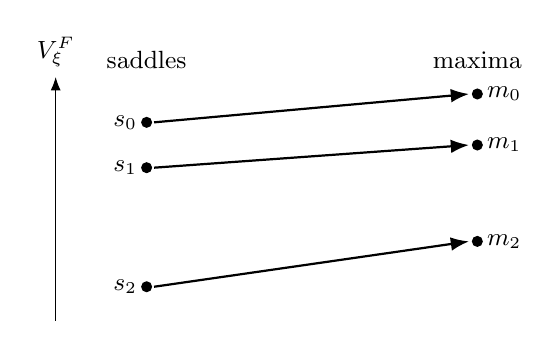
\begin{tikzpicture}[x=1.05cm,y=.72cm,>=Latex,
  every node/.style={font=\small}]
 \draw[->] (-1.1,0)--(-1.1,4.3) node[above] {$V^F_\xi$};
 \node at (0,4.6) {saddles};
 \node at (4,4.6) {maxima};
 \foreach \sy/\my/\r in {3.5/4/0,2.7/3.1/1,.6/1.4/2} {
  \draw[->,thick] (.09,\sy)--(3.9,\my);
  \fill (0,\sy) circle (2pt) node[left] {$s_{\r}$};
  \fill (4,\my) circle (2pt) node[right] {$m_{\r}$};
 }
\end{tikzpicture}
\caption{The first three ranks in a schematic good target fiber. Vertical
position records $V^F_\xi$; the two columns are ordered separately by decreasing
value, with lexicographic tie-breaking. Equal ranks are paired, and each arrow
ends at least as high as it starts.
The pole is absent from both lists, and additional maxima may remain unassigned.
Arrows describe the rank assignment, not curves in the source plane.}
\label{fig:rank-pairing}
\end{figure}


We give the Borel construction explicitly. Countable Borel enumeration
is the subject of the Lusin--Novikov theorem; see
\cite[4F.6 and 4F.17]{Moschovakis2009}. Here nonsingularity supplies
continuous local branches, and the rank definition will also supply
affine equivariance. Consider the nonsingular
solution graph
\[
 \Gamma=\{(F,\xi,w)\in\KK\times\CC\times\HH:
                    G_F(w)=\xi,\ J_F(w)\ne0\}.
\]
It can be covered by countably many continuous branches over open
parameter sets in $\KK\times\CC$.  To prove this without differentiating
in the parameter $F$, fix $(F_0,\xi_0,w_0)\in\Gamma$ and the invertible
real matrix $D=DG_{F_0}(w_0)$.  Joint continuity of derivatives on source
compacts gives a closed ball $\overline B(w_0,r)\subset\HH$ and an open
parameter neighborhood $U$ such that
\[
 \|I-D^{-1}DG_F(w)\|\le\frac12
 \quad(w\in\overline B(w_0,r)),\qquad
 |D^{-1}(G_F(w_0)-\xi)|<\frac r2
\]
for every $(F,\xi)\in U$.  The map
\[
 w\longmapsto w-D^{-1}(G_F(w)-\xi)
\]
is a contraction of the closed ball into its interior.  Its unique fixed
point exists by the contraction principle~\cite[Lemma~C.35]{Lee2013}.  This
point solves $G_F(w)=\xi$, is nonsingular, and depends continuously on
$(F,\xi)$.  Continuity follows, for instance, by taking any convergent
parameter sequence and using compactness of the ball and uniqueness to
identify every subsequential limit of its fixed points.

Consequently $\Gamma\cap(U\times B(w_0,r))$ is the graph of one
continuous branch over $U$, and is an open neighborhood in $\Gamma$.
The space $\Gamma$ is second countable, being a subspace of
$\KK\times\CC\times\HH$.  A countable collection of these branch
neighborhoods therefore covers it.  Enumerate the resulting continuous
partial branches as $b_j:U_j\to\HH$, $j\ge1$.
Activate branch $j$ at a parameter if the parameter is in $U_j$ and its
value differs from every earlier branch defined there.  These activation
sets are Borel: there are finitely many earlier indices for a given $j$,
and equality of two continuous branches is closed relative to their
open overlap.  Each nonsingular root occurs in exactly one active branch.

On a branch, its critical value can be evaluated without division by
$F(w)-\xi$, using the positive continuous function
\[
 H(F,w)=k(\operatorname{Im}w)^{k-1}|Q_F(w)|.
\]
At every root this equals $V^F_\xi(w)$ by
\eqref{eq:critical-height}.  The signs of $J_F$, comparisons of $H$,
equalities of values, and lexicographic comparisons of coordinates are
Borel.  The rank of an active branch among branches of its sign is thus
the countable sum of the Borel indicators of its active predecessors.
This is an extended-integer-valued Borel function, and is finite on good
fibers.  Requiring a positive-sign and a negative-sign active branch to
have the same finite rank gives a countable Borel test for the assigned
pair.

The set $\mathcal D$ is Borel by Lemma~\ref{lem:good-pairs} and continuity
of $(F,z)\mapsto(F,G_F(z))$.  At this target, require additionally that
the positive-sign branch equal $z$.  Exactly one active negative-sign
branch passes the equal-rank test, by the existence and uniqueness proved
above.  Selecting its value defines a Borel map on $\mathcal D$: the
preimage of an open source set is the countable union of the Borel tests
just described with the selected branch constrained to that set.

Finally, under the affine source change $w\mapsto t\cdot w$, the critical
fibers and signs correspond by
\eqref{eq:critical-map-covariance}--\eqref{eq:jacobian-covariance}.
All critical heights in a fiber are multiplied by the same positive
constant in \eqref{eq:critical-height-covariance}.  The positive real
source scale preserves lexicographic order, including ties of the first
coordinate.  Hence the two orders, their ranks, and the equal-rank
assignment correspond exactly, giving \eqref{eq:pairing-covariance}.
The enumeration was used only to prove measurability and does not enter
the geometric definition of the assignment.
\end{proof}

The ordering used in \eqref{eq:pairing-guarantees} also handles coincident critical values.
At each critical point, \eqref{eq:critical-height} and
$4(k-1)=\beta-1$ give
\begin{equation}
 y^{\beta-1}|Q_F(z)|^4
   =\left(\frac{V^F_\xi(z)}k\right)^4.
 \label{eq:critical-transport-weight}
\end{equation}
Thus the pairing increases the weight on the left of
\eqref{eq:critical-transport-weight}.  The next section uses this
pointwise comparison to contradict the positive expectation in
\eqref{eq:positive-jacobian-mean}.

\section{Transport between saddles and maxima}\label{sec:transport}

We now show that the weighted law obtained from $\rho>2$ is impossible.
The pairing of Proposition~\ref{prop:critical-pairing} compares masses
after changing variables by $G_F$.  Averaging that comparison over large
boxes will give $\EE J_F(i)\leq0$, contradicting
Lemma~\ref{lem:jacobian-moments}.

Throughout this section, suppose $\rho>2$, let
$\beta=\log_2\rho$ and $k=(\beta+3)/4$, and use the probability $P$ from
Lemma~\ref{lem:weighted-law}.  Write
\[
 J_{F,+}=\max(J_F,0),\qquad J_{F,-}=\max(-J_F,0),\qquad
 \omega_F(x+iy)=y^{\beta-1}|Q_F(x+iy)|^2.
\]
Recall that $\mathcal G\subset\KK\times\CC$ is the Borel set of good
pairs and that $R_F(z)$ is the assigned maximum whenever
$J_F(z)>0$ and $(F,G_F(z))\in\mathcal G$.

\subsection{Change of variables and exceptional targets}

For fixed $F$, the open set $\{J_F>0\}$ has a countable cover by open
sets on which $G_F$ is a diffeomorphism onto an open set.  Disjointifying
this cover gives Borel pieces $E_j$ on each of which $G_F$ is injective.
Their images are Borel: each restriction is contained in a
diffeomorphism chart, whose inverse is continuous.  Ordinary
absolute-Jacobian change of variables on these pieces, followed by
Tonelli's theorem \cite[Theorems~2.37 and~2.47]{Folland1999},
therefore gives change of variables with a sum over
preimages.  The same construction applies on $\{J_F<0\}$.
In particular, for every nonnegative Borel function $h$ on $\HH$,
\begin{equation}\label{eq:transport-area}
 \int_{\HH}\omega_F(z)J_{F,\pm}(z)h(z)\dd A(z)
 =
 \int_{\CC}
 \sum_{\substack{G_F(z)=\xi\\ \pm J_F(z)>0}}
 y^{\beta-1}|Q_F(z)|^4h(z)\dd A(\xi).
\end{equation}
Indeed, $|\det DG_F|=|F'|^2|J_F|$, so division by the absolute
Jacobian supplies the second factor $|Q_F|^2$.  All sums and integrals
in \eqref{eq:transport-area} are nonnegative; no global injectivity of
$G_F$ or finite total number of preimages is required.

The root target is $G_F(i)=-i/k$ for every $F$.  Since the exceptional
target set can depend on $F$, the almost-everywhere target assertion
in Lemma~\ref{lem:good-pairs} must still be transferred to this root.

\begin{lemma}[Exceptional targets at the root]\label{lem:root-exception}
 Suppose $\rho>2$, let $P$ be the weighted law of
 Lemma~\ref{lem:weighted-law}, and set
 $k=(\log_2\rho+3)/4$.  Then
 \begin{equation}\label{eq:root-exception}
  \EE\!\left[
   J_{F,+}(i)\,
   \mathbf 1_{\{(F,-i/k)\notin\mathcal G\}}
  \right]=0.
 \end{equation}
\end{lemma}

\begin{proof}
 For $P$-almost every $F$, the complement of
 $\{\xi:(F,\xi)\in\mathcal G\}$ has planar area zero by
 Lemma~\ref{lem:good-pairs}.  Apply \eqref{eq:transport-area} on the
 positive sign with
 \[
 h(z)=\mathbf 1_{B_0}(z)
       \mathbf 1_{\{(F,G_F(z))\notin\mathcal G\}},
 \qquad B_0=\{x+iy:|x|\leq1,\ 1\leq y\leq2\}.
 \]
 Its target integral is supported on that null set, so
 \begin{equation}\label{eq:exception-box}
  \int_{B_0}\omega_F(z)J_{F,+}(z)
   \mathbf 1_{\{(F,G_F(z))\notin\mathcal G\}}\dd A(z)=0
 \end{equation}
 for almost every $F$.

 Define the nonnegative Borel function
 \[
  \Phi(F)=J_{F,+}(i)
          \mathbf 1_{\{(F,-i/k)\notin\mathcal G\}}.
 \]
 The normalized Jacobian and goodness are affine-equivariant, so
 \[
  \Phi(T_zF)=J_{F,+}(z)
            \mathbf 1_{\{(F,G_F(z))\notin\mathcal G\}}.
 \]
 The weighted covariance identity consequently gives
 \[
  \EE[\omega_F(z)\Phi(T_zF)]
   =y^{\beta-1}y^{-\beta}\EE\Phi
   =y^{-1}\EE\Phi.
 \]
 Taking expectations in \eqref{eq:exception-box} and using Tonelli
 yields $0=2\log2\,\EE\Phi$, which proves the claim.
\end{proof}

\subsection{Box comparison and exhaustion}

For each positive integer $N$, let $D_N$ be the Borel set of pairs
$(F,z)$ for which $J_F(z)>0$, $(F,G_F(z))\in\mathcal G$, and the
assigned point $z'=R_F(z)=x'+iy'$ satisfies
\begin{equation}\label{eq:transport-displacement}
 \frac1N\leq\frac{y'}y\leq N,\qquad |x'-x|\leq Ny,
 \qquad z=x+iy.
\end{equation}
The Borel property follows from that of the pairing map.
Its equivariance gives
\begin{equation}\label{eq:transport-equivariance}
 \mathbf 1_{D_N}(F,z)=\mathbf 1_{D_N}(T_zF,i).
\end{equation}
The sets $D_N$ increase with $N$.  Every good-target saddle belongs
to some $D_N$, since its assigned point has finite coordinates and
strictly positive height.

Fix $R>0$ and $Y>1$, and put
\begin{align*}
 B_{R,Y}&=\{x+iy:|x|\leq R,\ 1\leq y\leq Y\},\\
 B'_{R,Y,N}&=\{x+iy:|x|\leq R+NY,\ 1/N\leq y\leq NY\}.
\end{align*}
If $z\in B_{R,Y}$ and $(F,z)\in D_N$, then
$R_F(z)\in B'_{R,Y,N}$ by \eqref{eq:transport-displacement}.
At a preimage $G_F(z)=\xi$, the critical-point identity gives
\begin{equation}\label{eq:transport-target-weight}
 y^{\beta-1}|Q_F(z)|^4
   =\left(\frac{V^F_\xi(z)}k\right)^4,
 \qquad 4(k-1)=\beta-1.
\end{equation}
The pairing is injective on each target fiber, and its assigned
maximum has at least the saddle's $V$-value.  Applying
\eqref{eq:transport-area} to both signs and comparing the target
sums with \eqref{eq:transport-target-weight} therefore proves
\begin{equation}\label{eq:transport-box}
 \int_{B_{R,Y}}\omega_FJ_{F,+}\mathbf 1_{D_N}\dd A
 \leq
 \int_{B'_{R,Y,N}}\omega_FJ_{F,-}\dd A.
\end{equation}
This inequality holds for every $F$; the left side selects only
fibers on which the pairing is defined.
Both source integrands are jointly Borel and nonnegative in $(F,z)$,
so Tonelli's theorem applies when we average this fixed-$F$ inequality.

\begin{proposition}[Transfer bound]\label{prop:transfer-bound}
 The dyadic transfer operator satisfies $\rho\leq2$.
\end{proposition}

\begin{proof}
 Continue under the contrary assumption $\rho>2$.  By weighted
 covariance and \eqref{eq:transport-equivariance},
 \[
 \EE[\omega_F(z)J_{F,+}(z)\mathbf 1_{D_N}(F,z)]
  =y^{-1}\EE[J_{F,+}(i)\mathbf 1_{D_N}(F,i)].
 \]
 Likewise $\EE[\omega_F(z)J_{F,-}(z)]=y^{-1}\EE J_{F,-}(i)$.
 Thus expectation in \eqref{eq:transport-box} yields
 \begin{equation}\label{eq:transport-expected-box}
 \begin{split}
 2R\log Y\,
   \EE[J_{F,+}(i)\mathbf 1_{D_N}(F,i)]
 \leq{}&
 2(R+NY)\log(N^2Y)\,\EE J_{F,-}(i).
 \end{split}
 \end{equation}
 The root quantities are integrable: $q_F(i)$ is uniformly bounded
 on the compact normalized class, and $J_F(i)$ is a fixed quadratic
 expression in this jet.

 Hold $N$ fixed, set $R=Y^2$, and let $Y\to\infty$.  The ratio of the
 right box factor to the left one is
 \[
  \left(1+\frac NY\right)
  \left(1+\frac{2\log N}{\log Y}\right)\longrightarrow1.
 \]
 Dividing \eqref{eq:transport-expected-box} by $2R\log Y$ gives
 \[
  \EE[J_{F,+}(i)\mathbf 1_{D_N}(F,i)]\leq\EE J_{F,-}(i).
 \]
 Now let integer $N\to\infty$.  Monotone convergence exhausts the
 good-target saddles, and Lemma~\ref{lem:root-exception} accounts for
 the remaining positive-J weight.  Hence
 \[
  \EE J_{F,+}(i)\leq\EE J_{F,-}(i),\qquad \EE J_F(i)\leq0.
 \]
 For the same $J_F$ and the same law $P$,
 Lemma~\ref{lem:jacobian-moments} gives
 \[
  k^2\EE J_F(i)
  =k(k-1)-(2k-1)\frac{\beta}{2}
                   +\frac{\beta(\beta+1)}4
  =k(k-1)>0,
 \]
 since $2k-1=(\beta+1)/2$ and $k>1$.  This contradiction proves
 $\rho\leq2$.
\end{proof}

\section{Integral means and the full integrability range}
\label{sec:integrability}

Proposition~\ref{prop:transfer-bound} and the disk comparison now
give the inverse-square estimate.  We first identify its sharp
integral-means exponent, then obtain the negative area exponents by
H\"older's inequality.  The positive exponents follow from a
separate weighted area estimate for univalent maps.

\subsection{The inverse-square endpoint and negative powers}

\begin{proof}[Proof of the integral-means assertion in Theorem~\ref{thm:main}]
 Proposition~\ref{prop:transfer-bound} gives $\rho\leq2$.
 Proposition~\ref{prop:disk-transfer} therefore implies that, for every
 $\epsilon>0$, there is $C_\epsilon<\infty$, independent of
 $f\in\SSS$, such that
 \begin{equation}\label{eq:final-inverse-means}
  M_{-2}[f'](r)\leq C_\epsilon(1-r)^{-1-\epsilon},
  \qquad \frac12\leq r<1.
 \end{equation}
 In particular $\beta_f(-2)\leq1$ for every $f\in\SSS$.

 For the reverse inequality consider the Koebe map
 \[
  f_{\mathrm K}(z)=\frac{z}{(1-z)^2},\qquad
  f_{\mathrm K}'(z)=\frac{1+z}{(1-z)^3}.
 \]
 It belongs to $\SSS$: equality of its values at $z,u\in\DD$
 gives $(z-u)(1-zu)=0$, hence $z=u$.
 Write $\delta=1-r$ and take $r$ sufficiently close to $1$.
 On the arc $z=re^{i(\pi+\theta)}$ with $|\theta|\leq\delta$,
 \[
  |1+z|\leq\delta+r|\theta|\leq2\delta,\qquad |1-z|\geq1.
 \]
 Consequently
 \[
  M_{-2}[f_{\mathrm K}'](r)
    \geq \frac1{2\pi}\int_{-\delta}^{\delta}
                      \frac{d\theta}{4\delta^2}
    =\frac1{4\pi\delta}.
 \]
 No exponent smaller than $1$ can bound these means near the
 boundary.  Hence $\beta_{f_{\mathrm K}}(-2)\geq1$, and
 $B_{\SSS}(-2)=1$.
\end{proof}

\begin{corollary}[The full negative linear tail]\label{cor:negative-linear-tail}
For every real $t\leq-2$ and every $\epsilon>0$, there is
$C_{t,\epsilon}<\infty$ such that
\begin{equation}\label{eq:negative-linear-tail}
 M_t[f'](r)\leq C_{t,\epsilon}(1-r)^{-(|t|-1)-\epsilon}
 \qquad\left(f\in\SSS,\ \frac12\leq r<1\right).
\end{equation}
Consequently,
\[
 B_{\SSS}(t)=|t|-1\qquad(t\leq-2).
\]
\end{corollary}

\begin{proof}
Put $a=|t|-2\geq0$.  The distortion lower bound
\eqref{prelim:disk-bounds} and \eqref{eq:final-inverse-means} give
\[
 \begin{aligned}
 M_t[f'](r)
 &\leq\left(\frac{(1+r)^3}{1-r}\right)^a M_{-2}[f'](r)\\
 &\leq 8^a C_\epsilon(1-r)^{-(a+1)-\epsilon}.
 \end{aligned}
\]
Since $a+1=|t|-1$, this proves \eqref{eq:negative-linear-tail} with
$C_{t,\epsilon}=8^{|t|-2}C_\epsilon$.  At $t=-2$ it is exactly
\eqref{eq:final-inverse-means}.  For each fixed $f$ and $t$, letting
$\epsilon\downarrow0$ in the definition of $\beta_f(t)$ gives
$\beta_f(t)\leq|t|-1$; taking the supremum over $f$ gives the same
upper bound for $B_{\SSS}(t)$.

For the Koebe map and the arc used above, $|f_{\mathrm K}'(z)|\leq2\delta$.
Thus, for $\delta=1-r$ sufficiently small,
\[
 M_t[f_{\mathrm K}'](r)
 \geq\frac1{2\pi}\int_{-\delta}^{\delta}(2\delta)^{-|t|}\,d\theta
 =\frac{2^{-|t|}}{\pi}\delta^{1-|t|}.
\]
Hence $\beta_{f_{\mathrm K}}(t)\geq|t|-1$, proving the equality.
\end{proof}

For $-2<t<0$, put $q=-t/2\in(0,1)$.  H\"older's inequality on the
probability circle gives
\begin{equation}\label{eq:negative-holder}
 M_t[f'](r)
   =\frac1{2\pi}\int_{-\pi}^{\pi}
        \bigl(|f'(re^{i\theta})|^{-2}\bigr)^q\dd\theta
   \leq M_{-2}[f'](r)^q.
\end{equation}
Choose $0<\epsilon<1/q-1$.  The exponent $q(1+\epsilon)$ in
\eqref{eq:final-inverse-means} is then less than $1$, so
\begin{equation}\label{eq:negative-area}
 \int_{\DD}|f'|^t\dd A
    =2\pi\int_0^1 r M_t[f'](r)\dd r<\infty
    \qquad(f\in\SSS,\ -2<t<0).
\end{equation}
There is no singularity on a compact subdisk because $f'$ never
vanishes.  The case $t=0$ gives the area $\pi$.

\subsection{Positive powers}

We use the classical bounds of Lemma~\ref{lem:classical-univalence}
to establish two elementary integrability statements for $f$ itself.

\begin{lemma}[Function means and area powers]\label{lem:function-powers}
 For every $0<p<1/2$ there is $C_p<\infty$ such that
 \begin{equation}\label{eq:function-means}
  \frac1{2\pi}\int_{-\pi}^{\pi}
       |f(re^{i\theta})|^p\dd\theta\leq C_p
  \qquad(f\in\SSS,\ 0<r<1).
 \end{equation}
 Moreover, for every $0\leq a<1$ and every $f\in\SSS$,
 \begin{equation}\label{eq:function-area}
  \int_{\DD}(1+|f(z)|)^a\dd A(z)<\infty.
 \end{equation}
\end{lemma}

\begin{proof}
 Away from the simple zero of $f$ at $0$,
 \[
  \Delta |f|^p=p^2|f|^{p-2}|f'|^2.
 \]
 The right side is locally integrable also at $0$, where it is
 $O(|z|^{p-2})$.  Green's radial mean identity gives
 \begin{equation}\label{eq:function-green}
 \frac1{2\pi}\int_{-\pi}^{\pi}|f(re^{i\theta})|^p\dd\theta
 =\frac{p^2}{2\pi}\int_{|z|<r}
   |f(z)|^{p-2}|f'(z)|^2\log\frac r{|z|}\dd A(z).
 \end{equation}
 To justify it at the zero, apply Green's theorem on an annulus
 \cite[Theorem~16.17]{Lee2013} with
 inner radius $\delta$.  The circular mean at that radius is
 $O(\delta^p)$ and its derivative is $O(\delta^{p-1})$, because
 $f(z)=z+O(z^2)$.  The inner terms are consequently
 $O(\delta^p(1+|\log\delta|))$ and vanish as $\delta\downarrow0$.

 Bound the logarithm in \eqref{eq:function-green} by
 $\log(1/|z|)$.  On $|z|\leq1/2$, the classical bounds give
 $|f(z)|\geq c|z|$ and $|f'(z)|\leq C$, uniformly in $\SSS$.
 Since $p-2<0$, this part is bounded by a constant times
 \[
  \int_0^{1/2}u^{p-1}\log(1/u)\dd u<\infty.
 \]
 On $|z|>1/2$, the growth bound
 $|f(z)|\leq |z|/(1-|z|)^2$ implies
 \[
  \log\frac1{|z|}
   \leq C(1-|z|)
   \leq C\min\{1,|f(z)|^{-1/2}\}.
 \]
 The conformal change of variables $w=f(z)$ therefore bounds the
 remaining integral by a constant times
 \[
  \int_{\CC}|w|^{p-2}\min\{1,|w|^{-1/2}\}\dd A(w)
  =2\pi\left(\int_0^1u^{p-1}\dd u
             +\int_1^\infty u^{p-3/2}\dd u\right)<\infty.
 \]
 This proves \eqref{eq:function-means}.

 For \eqref{eq:function-area}, the case $a=0$ is immediate.
 For $0<a<1$, choose
 \[
   \max\{0,a-\tfrac12\}<p<\tfrac12.
 \]
 If $a\leq p$, the power-mean inequality and
 \eqref{eq:function-means} bound the means of $|f|^a$.
 If $a>p$, the growth bound gives instead
 \[
  \frac1{2\pi}\int_{-\pi}^{\pi}|f(re^{i\theta})|^a\dd\theta
   \leq
   \left(\max_{|z|=r}|f(z)|\right)^{a-p}C_p
   \leq C_p(1-r)^{-2(a-p)}.
 \]
 Thus the means of $(1+|f|)^a$ are bounded by
 $C(1-r)^{-2(a-p)_+}$, where $(b)_+=\max\{b,0\}$.
 Since $2(a-p)_+<1$, radial integration proves the claim.
\end{proof}

\begin{lemma}[Positive derivative powers]\label{lem:positive-derivative-powers}
 For every $f\in\SSS$ and $0<t<2/3$,
 \[
  \int_{\DD}|f'(z)|^t\dd A(z)<\infty.
 \]
\end{lemma}

\begin{proof}
 Choose $0<\eta<2/t-3$ and set
 \[
  a=\frac{(2+\eta)t}{2-t}\in(0,1),\qquad
  u_\eta(z)=|f'(z)|^2(1+|f(z)|)^{-2-\eta}.
 \]
 Injective conformal area change gives
 \begin{equation}\label{eq:weighted-derivative-area}
  \int_{\DD}u_\eta\dd A
   =\int_{f(\DD)}(1+|w|)^{-2-\eta}\dd A(w)
   \leq\frac{2\pi}{\eta(1+\eta)}.
 \end{equation}
 Here the last constant is the polar integral over $\CC$.
 The exact factorization
 \[
  |f'|^t=u_\eta^{t/2}\bigl((1+|f|)^a\bigr)^{(2-t)/2}
 \]
 and H\"older's inequality with exponents $2/t$ and $2/(2-t)$
 now yield
 \[
  \int_{\DD}|f'|^t\dd A
   \leq
    \left(\int_{\DD}u_\eta\dd A\right)^{t/2}
    \left(\int_{\DD}(1+|f|)^a\dd A\right)^{(2-t)/2}<\infty
 \]
 by Lemma~\ref{lem:function-powers}.
\end{proof}

\subsection{Domains, equivalence, and endpoint sharpness}

\begin{proof}[Proof of the area assertion in Theorem~\ref{thm:main}]
 Equations~\eqref{eq:negative-area} and
 Lemma~\ref{lem:positive-derivative-powers}, together with $t=0$,
 prove the disk integral for $f\in\SSS$ throughout
 $-2<t<2/3$.  For an arbitrary univalent $f:\DD\to\CC$,
 \[
  g(z)=\frac{f(z)-f(0)}{f'(0)}\in\SSS,\qquad
  \int_{\DD}|f'|^t\dd A
    =|f'(0)|^t\int_{\DD}|g'|^t\dd A.
 \]
 The multiplier is finite and positive for every real $t$.

 If $\varphi:W\to\DD$ is a conformal bijection and
 $f=\varphi^{-1}$, the identities
 $\varphi'(f(w))=1/f'(w)$ and
 $\dd A(f(w))=|f'(w)|^2\dd A(w)$ give
 \begin{equation}\label{eq:domain-change}
  \int_W|\varphi'(z)|^s\dd A(z)
    =\int_{\DD}|f'(w)|^{2-s}\dd A(w).
 \end{equation}
 This change of variables is valid for nonnegative integrands,
 whether or not the integrals are finite.  Since
 $4/3<s<4$ is equivalent to $-2<2-s<2/3$, the desired domain
 integral is finite.
\end{proof}

For completeness, the disk and domain formulations have exactly
the same scope.  A univalent disk image is simply connected and
cannot equal $\CC$, since its inverse would be a bounded entire
nonconstant function.  If its boundary in the sphere had at most
one point, it would be a nonempty clopen subset of the connected
sphere with that possible point removed.  It would therefore be
the whole sphere or a punctured sphere, which is incompatible
with being a proper plane domain.  Thus it satisfies the stated
boundary-size condition, and \eqref{eq:domain-change} applies to
its inverse.  Conversely, each conformal bijection in the domain
formulation has a univalent inverse on $\DD$.

For a plane domain $U$ and $1\leq r\leq\infty$, write $L_r^1(U)$
for the homogeneous Sobolev space of locally integrable, weakly
differentiable real-valued functions with seminorm
$\|\nabla u\|_{L^r(U)}<\infty$, using the essential supremum when
$r=\infty$.

\begin{corollary}[Homogeneous Sobolev pullback]\label{cor:sobolev-pullback}
 Let $\Omega\subset\CC$ be a simply connected domain whose boundary
 in the Riemann sphere has at least two points, and let
 $\varphi:\Omega\to\DD$ be a
 conformal bijection. For $2<p<\infty$ and $4/3<s<4$, put
 $q=ps/(p+s-2)$. Then pullback $\varphi^*u=u\circ\varphi$ is bounded
 from $L_p^1(\DD)$ to $L_q^1(\Omega)$. It is also bounded from
 $L_\infty^1(\DD)$ to $L_s^1(\Omega)$ for every $4/3<s<4$.
 The finite bounds on gradient seminorms may depend on the map and
 the exponents.
\end{corollary}

\begin{proof}
 This is the known Sobolev formulation of Brennan's conjecture due to
 Gol'dshtein and Ukhlov
 \cite[Equivalence Theorem and its following Remark~2]{GoldshteinUkhlov2013}.
 Indeed, $1<q<p$ and $(p-2)q/(p-q)=s$, so Theorem~\ref{thm:main}
 supplies the derivative integrability required by their equivalence.
 The cited remark gives the case $p=\infty$, with $q=s$.
\end{proof}

The area assertion also implies the individual endpoint
integral-means bound.  Indeed, fix $f\in\SSS$ and $0<\eta<2$.
The function $|f'|^{-2+\eta}$ is subharmonic, since $f'$ is
nonvanishing; hence its circular means $M_{-2+\eta}[f'](r)$
are nondecreasing.  If its disk area integral is finite, then,
for $r\geq1/2$,
\[
 \int_{\DD}|f'|^{-2+\eta}\dd A
 \geq2\pi M_{-2+\eta}[f'](r)\int_r^1u\dd u,
\]
so $M_{-2+\eta}[f'](r)\leq C_{f,\eta}(1-r)^{-1}$.
The distortion lower bound gives
$|f'(re^{i\theta})|^{-\eta}\leq C_\eta(1-r)^{-\eta}$.
Multiplying these bounds yields
\[
 M_{-2}[f'](r)\leq C'_{f,\eta}(1-r)^{-1-\eta}.
\]
Letting $\eta\downarrow0$ in the definition of the exponent gives
$\beta_f(-2)\leq1$.  In the other direction, this individual
exponent bound gives an estimate with every positive exponent
loss, and \eqref{eq:negative-holder} gives all negative interior
area exponents.  The positive exponents were proved independently
above.  Together with the Koebe lower bound, this establishes the
stated equivalence with $B_{\SSS}(-2)=1$.  In our proof, the uniform constant in
\eqref{eq:final-inverse-means} comes directly from the transfer-operator
argument.

\begin{proof}[Proof of Corollary~\ref{cor:sharp-endpoints}]
 Use the same Koebe map $f_{\mathrm K}$.  For sufficiently small
 $|w|$,
 \[
  |f_{\mathrm K}'(-1+w)|=\frac{|w|}{|2-w|^3}\asymp |w|,
  \qquad
  |f_{\mathrm K}'(1-w)|=\frac{|2-w|}{|w|^3}\asymp |w|^{-3}.
 \]
 The fixed sector
 \[
  0<|w|<\tfrac12,\qquad |\arg w|<\tfrac{\pi}{3}
 \]
 lies inside $\DD$ under either substitution $z=-1+w$ or
 $z=1-w$: in both cases $|z|^2=1-2\Re w+|w|^2<1$.
 The area integral at $t=-2$ near $-1$ and the one at $t=2/3$
 near $1$ therefore each dominate a positive multiple of
 \[
  \int_0^{1/2}u^{-2}u\dd u=\infty.
 \]
 More generally these sectors diverge for $t\leq-2$ and
 $t\geq2/3$, respectively.  The image of $f_{\mathrm K}$ meets
 the domain hypotheses just verified, so its inverse, by
 \eqref{eq:domain-change}, also gives divergence at $s=4$ and
 $s=4/3$.  Thus both open endpoints are sharp.
\end{proof}

\bibliographystyle{alphaurl}
\bibliography{references/references}
\end{document}
